\documentclass[12pt,a4paper]{IEEEtran}
\usepackage[margin=0.65in]{geometry}
\usepackage[affil-it]{authblk}
\usepackage{graphicx}
\usepackage[table,xcdraw]{xcolor}
\usepackage{caption}
\usepackage{subcaption}
\usepackage{float}
\usepackage{hyperref}
\usepackage{relsize}
\usepackage{textcomp}
\usepackage{placeins}
\usepackage{kbordermatrix,amsmath}
{
	%	\theoremstyle{plain}
	\newtheorem{assumption}{Assumption}
}
\usepackage[most]{tcolorbox}
\tcbset{textmarker/.style={%
		enhanced,
		parbox=false,boxrule=0mm,boxsep=0mm,arc=0mm,
		outer arc=0mm,left=6mm,right=3mm,top=7pt,bottom=7pt,
		toptitle=1mm,bottomtitle=1mm}}

\newtcolorbox{importantBox}{textmarker,
	borderline west={6pt}{0pt}{red},
	colback=red!10!white}

\newcommand{\important}[1]{\begin{importantBox} \textbf{Important:} #1 \end{importantBox}}
\newcommand{\magn}[1]{\Vert{#1}\Vert}
\newcommand{\card}[1]{\vert{#1}\vert}
%\newcommand{\vbb}[2]{\vec{#1#2}}
\newcommand{\vbb}[2]{#2-#1}
%\renewcommand{\vec}[1]{\overrightarrow{#1}}
\newcommand{\pangle}{\mathit{\alpha}}
\newcommand{\leqaz}[3]{#2 \leq_{\pangle_#1} #3}
\newcommand{\angleordered}[2]{\langle #2 \rangle_{\leqaz{#1}{}{}}}
\newcommand{\prm}{\mathsf{prm}}
\newcommand{\kc}{\mathit{k_{c}}}
\newcommand{\kr}{\mathit{k_{r}}}
\newcommand{\kd}{\mathit{k_{d}}}
\newcommand{\kg}{\mathit{k_{g}}}
\newcommand{\ko}{\mathit{k_{o}}}
\newcommand{\rb}{\mathit{R}}
\newcommand{\rgf}{\mathit{rgf}}
\title{A Novel Relationship-based Approach to Swarm Coordination.}
\author[*]{Neil Eliot}
\author[ ]{David Kendall}
\author[ ]{Michael Brockway}
\author[ ]{Paul Oman}
\author[ ]{Ahmed Bouridane}
\affil[ ] {Department of Computer Sciences, Northumbria University}
\affil[*] {Corresponding author: Dr Neil Eliot, neil.eliot@northumbria.ac.uk}
\date{\today}


\begin{document}
\maketitle

\begin{abstract}
Currently, most of the models for swarm coordination are based upon fixed (single value) potential fields. Although, this approach enables predictable behaviours to be created and simplifies the underpinning model, it limits the control of an agent’s movement by treating all agents equally. To allow a more configurable model the agent’s perimeter status and the status of each neighbour can be considered when applying coordination parameters.  This paper proposes a novel model to swarm coordination using a relationship-based approach to enable emergent behaviours to be created resulting in a much-improved structure of a swarm thus making it applicable to specific applications such as reconnaissance problems where a high-density swarm frontier and/or a reduced perimeter density may be required at the frontier. The model is based upon perimeter identification of the structure the use of an agent’s perimeter status as an alternative controlling dynamic can be induced.
The movement can be modified using three arrays indexed by the agent’s status while the agent’s vector calculations are modified by these array entries to produce the final movement vector. Extensive experiments were carried out to demonstrate how the new model can implement various behaviours such as packed and expanded perimeters to emerge for a random swarm deployment and how the new model can still operate as the traditional single value potential field model. The results show that by modifying the generated vectors of agents based upon their relationships several novel swarming behaviours can easily be produced, such as void removal, perimeter packing and expansion and can be tailored to relevant swarming applications.
\end{abstract}

\section{Introduction}
When cohesion and repulsion field effects (sometimes referred to as potential fields~\cite{BAF:06,eliot2018metric,VG:05,liang2019swarm,SW:03,Son2017}) are used to create a swarming effect, the stable structures that develop are limited to either straight edges or partial lattices \cite{eliot2017methods}. The maintenance of a well-structured swarm is crucial to effective deployment for applications such as reconnaissance and artificial pollination, where `blind spots' are best eliminated \cite{elamvazhuthi2015optimal}, and containment, where the swarm is used to surround an object or region \cite{cao2012distributed}. Over time swarms form regular shapes~\cite{RAZ:13} and perimeters form of partial lattices that may contain so-called \textit{anomalies}, such as concave `dents' or convex `peaks'~\cite{eliot2019void}. These anomalies contribute to the disruption of an otherwise well-structured swarm. The key, therefore, is to ensure that these \textit{anomalies} are dynamically removed from a swarm whilst maintaining a regular formation.\\
To allow the new behaviours to be realised, such as creating a `pull' effect between perimeter agents to allows a swarm to remove anomilies, perimeter agent identification is required. This is discussed by Eliot et. al. in \cite{eliot2017methods, eliot2018metric, eliot2019void} and in Section~\ref{sec:perimeterDetection}.\\
The aim of the new model presented in this paper is to create a flexible relationship-based coordination technique that allows new emergent behaviours to be created by modifying the inter-agent weightings and field sizes. Figure \ref{fig:stableswarm}) shows an agent and it fields. $P$ is the perception field (The range of the sensor array). $O$ is the obstacle field. $C$ is the cohesion field and $\rb$ is the repulsion field. The new model involves introducing three controlling arrays to the existing potential field model; $\kc$ which modifies the magnitude of the cohesion vector. $\kr$ which modifies the repulsion vector and $\rb$ which alters the repulsion field.\\

\begin{figure}[H]
	\centering
	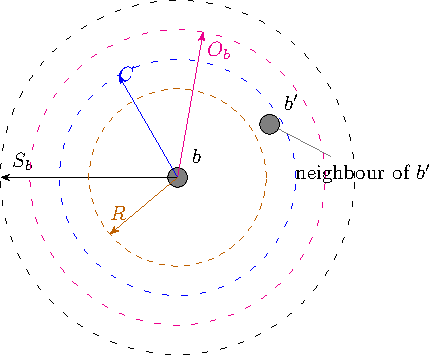
\includegraphics[width=0.7\linewidth]{figures/stableswarm}
	\caption[Agent Fields]{Agent Fields}
	\label{fig:stableswarm}
\end{figure}
%\FloatBarrier

\section{Related work}
As far back as 1987 swarm theory has adopted the use of potential fields to coordinate agents~\cite{REY:87} and this has continued since then in an attempt to improve the structure of a swarm, coordinate obstacle avoidance, and improve navigation~\cite{BAFVM:06,BAF:06,BFV:07,BM:09,eliot2018metric,VG:05,HC:09,SW:03,Son2017}. Improvements to the basic structure of swarms has developed through the likes of a prototype framework for self-healing swarms that was developed by Dai et al. where they consider how to manage agent failure in hostile environments \cite{DHMRZ:06}. This was similar to work by Vassev and Hinchey, who modelled swarm movement using the ASSL (Autonomic System Specification Language) \cite{VH:09}. This technique was employed by NASA (US National Aeronautics and Space Administration) for use in asteroid belt exploration as part of their ANTS (Autonomous Nano Technology Swarm) project. However, this work is focused towards failure of an agent's internal systems, rather than on the removal of anomalies in agent distribution. 

In the context of swarm structure maintenance, the need for formation control is discussed by Speck and Bucci with respect to the diverse applications of swarms and the need to control a swarms structure~\cite{8430773}. Roach et al. focusses on the effects of sensor failure, and the impact that has on agent distribution \cite{RMT:15}. Lee and Chong identified the issue of concave edges within swarms in an attempt to create regular lattice formations \cite{GN:08}, the main focus of their work is the dynamic restructuring of inter-agent formations. Ismail and Timmis demonstrated the use of \textit{bio-inspired} healing using \textit{granuloma formation}, a biological method for encapsulating an antigen \cite{IT:10}. They also considered the effect failed agents can have on a swarm when traversing a terrain~\cite{TIBW:16}. Jung et al. proposed a mediator-based approach using monolithic agents~\cite{6766522}. However, the formations are `controlled' by a human and not truly emergent behaviours. Karthikeyan and Ali proposed a communications-based technique to create specific shapes in a defined euclidean space such as lines, circles and triangles\cite{karthikeyan2006general}. Bruemmer et al. also proposed shape forming swarms but again using a communications-based methodology~\cite{bruemmer2002robotic}. Meng et al. use a bio-inspired technique to create swarm formation~\cite{meng2013morphogenetic}. However, the shapes are predetermined for the agents to migrate towards. He et al. also proposed a formation control mechanism which is communications-based~\cite{he2018feedback}. Fedele and D'Alfonso proposed a model for swarm structure control but it assumes `with out delay' communications-based architecture~\cite{8263694}. Fedele and D'Alfonso also proposed a matrix-based coordination algorithm to modify the movement of a swarms agents allowing shape formation in a fixed 3D environment~\cite{fedele2021coordinates}.

This paper proposes an alternative approach to agent coordination that can be used to induce, among other behaviours, perimeter expansion, packing and a void reduction effect in a unbounded Euclidean plane. This is an extension of the work presented by Eliot et al. \cite{eliot2019void}, Ismail and Timmis~\cite{IT:10,TIBW:16}, and on the work of McLurkin and Demaine on the detection of perimeter types~\cite{mclurkin2009}. However, perimeter type identification requires a communications infrastructure to allow the perimeter angle to be calculated. Communications within swarm formations limits swarm sizes and introduces performance problems~\cite{fu2020formation}. The technique employed in this paper does not explicitly require the identification of the perimeter type as it would limit the size of the swarm~\cite{eliot2019void,GN:08} and is therefore a reduced perimeter detection algorithm to identify \textit{any} perimeter.

\section{Basic swarming model}\label{sec:basicModel}
In the work by Eliot et. al. the resultant vector of an agent was calculated using Equation~\ref{eq:resultantVector1a}. Where $\kc, \kr, k_d, k_o$ are weighting factors for the summed vectors associated with each interaction. i.e. $v_c$, $v_r$, $v_d$, $v_o$ for cohesion, repulsion, direction and object avoidance respectively. 

\begin{equation}\label{eq:resultantVector1a}
	v(b) = \kc v_c(b) + \kr v_r(b) + \kd v_d(b) + \ko v_o(b)
\end{equation}

Equation~\ref{eq:resultantVector1a} shows the movement vector as a linear combination of a cohesion vector $v_c$ tending to move $b$ towards its neighbours, a repulsion vector $v_r$ tending to move $b$ away from its neighbours, a direction vector  $v_d$ tending to move $b$ towards a goal, and a vector $v_o$ tending to steer it away from obstacles. $\kc, \kr, ...$ are the scalar coefficients of the the linear combination.

This paper does not consider goals or obstacles so we assume $\kd = \ko = 0$ and omit the third and fourth terms.

\subsection{Cohesion}\label{cohesion}
The cohesion component is calculated based on the proximity of neighbours. Where $n_c(b)$ is the set of neighbour agents for $b$ (Eq. \ref{eq:cohesion1}). The inclusion of an agent from a swarm ($S$) in the neighbour set is achieved using the agent's cohesion field ($C$).

\begin{equation}\label{eq:cohesion1}
n_c(b) = \{b' \in S~:~b' \neq b \land\magn{\vbb{b}{b'}} \leq C\}
\end{equation}

The effect of an agent being within this set is that it will generate a vector that should `encourage' an agent to maintain their proximity. When there are multiple neighbours the cohesion effect is cumulative as shown by equation~\ref{eq:cohesion2} which creates a vector towards the centre of an agent's neighbours, creating a cohesive swarm. $\card{n_c(b)}$ denotes the cardinality of $n_c(b)$. This is the component of the overall vector calculation that has the $\kc$ quotient applied to it to allow the cohesion effect to be `balanced' with respect to other vector influences as described in ~\cite{eliot2017methods,eliot2018metric,eliot2019void}. 

\begin{equation}\label{eq:cohesion2}
v_c(b) = \frac{1}{\card{n_c(b)}} \sum_{b' \in n_c(b)}(\vbb{b}{b'})
\end{equation}

\subsection{Repulsion}\label{repulsion:neighbours}
The repulsion component of an agent's movement is derived from its interaction with its repulsion neighbours $n_r(b)$ (Eq.~\ref{eq:repulsion1a}) in a swarm ($\mathcal{S}$). Repulsion neighbours are identified as agents that are within the agent's ($b$) repulsion field ($\rb$).

\begin{equation}\label{eq:repulsion1a}
n_r(b) = \{b' \in \mathcal{S} : b \neq b' \land \card{\vbb{b}{b'}} \leq \rb\}
\end{equation}

The repulsion is then calculated as the average of all the vectors created by the agent ($b$) to the neighbours ($b'$) (Eg.~\ref{eq:repulsion2a}) and its proximity ($\magn{\vbb{b}{b'}} - \rb$). Where $\card{n_r(b)}$ denotes the cardinality of $n_r(b)$. This vector is then scaled to `balance' the effect as shown is Equation~\ref{eq:resultantVector1a} where $\kc$ is applied.

\begin{equation}\label{eq:repulsion2a}
v_r(b) = \frac{1}{\card{n_r(b)}}\sum_{b' \in n_r(b)} \left(1 - \frac{R}{\magn{\vbb{b}{b'}}} \, \right)\left(\vbb{b}{b'}\right)
\end{equation}

\section{New Inter-agent Model}
In this paper, we propose that the behaviour of an agent should be modified depending on its relationship with a neighbour using the status of whether or not it is on a \emph{perimeter} agent. Figure~\ref{fig:simplePerim2} shows a simple swarm. Perimeter agents are highlighted in \textcolor{red}{red} and can form part of an inner or outer boundary. A swarm can also contain non-perimeter agents which are shown in black.

\begin{figure}[H]
	\begin{center}
		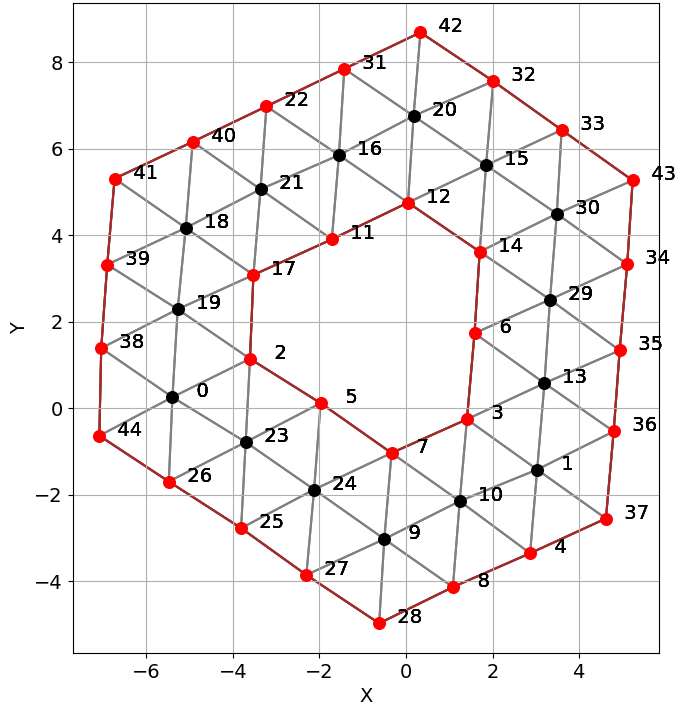
\includegraphics[width=0.8\linewidth]{figures/relationships2}
	\end{center}
	\caption{Outer and inner swarm perimeters. \label{fig:simplePerim2}}
\end{figure}
%\FloatBarrier

\subsection{Perimeter detection}\label{sec:perimeterDetection} 

Each agent's perimeter status is identified using a cyclic analysis of its cohesion neighbours~(Fig.~\ref{fig:neighbours3}). Ghrist et al. discuss a similar technique using sweep angles~\cite{ghrist2008surrounding} as do McLurkin et al~\cite{mclurkin2009}. 

We order the cohesion neighbours of an agent $b$ by their \emph{polar angle} ($\alpha$) with respect to $b$ (Fig.~\ref{fig:neighbours3}). 

The polar angle with respect to $b$ of a neighbour, $b'$, $\pangle(b, b')$, is the counter-clockwise angle that vector $\vec{bb'}$ makes with the positive $x$ axis, shown in Figure~\ref{fig:neighbours3} as $\alpha_i$ and defined by Equation~\ref{eq:pangle}.

\begin{align}\label{eq:pangle}
	& \pangle(b, b') = \theta~\mathrm{where}   \nonumber \\
	&		\quad~\land~0 \leq \theta < 2\pi \nonumber \\
	&   \quad~\land~\|b'-b\|(\cos\theta,\sin\theta) = b'- b 
\end{align} 

\begin{figure}[H]
	\centering
	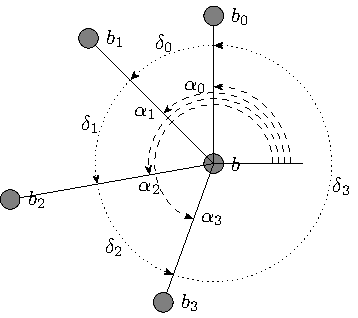
\includegraphics[width=0.8\linewidth]{figures/neighbours3}
	\caption[Agent neighbours]{Agent neighbour angles: {\small
	 $\alpha_0 = \pangle(b, b_0)$, $\alpha_1 = \pangle(b, b1)$, \ldots and
	 $\delta_0 = \pangle(b, b_1) - \pangle(b, b_0)$, $\delta_1 = \pangle(b, b_2) - \pangle(b, b_1)$, \ldots}}
	\label{fig:neighbours3}
\end{figure}
%\FloatBarrier

We denote by $\angleordered{b}{b_0, b_1, .., b_{n-1}}$ a permutation of the set of
neighbours, $n_c(b)$, that is sorted in non-decreasing order of \emph{polar angle}, i.e.
$\pangle(b, b_0) \leq \pangle(b, b_1) \leq \cdots \leq \pangle(b, b_{n-2}) \leq \pangle(b, b_{n-1})$.

An agent $b$ is on a perimeter if it satisfies any one of three conditions:
\begin{enumerate}
	\item consecutive neighbours are not within each other's cohesion field, or
	\item consecutive neighbours subtend a reflex angle (shown in Figure~\ref{fig:neighbours3} as $\delta_3$), or
	\item the agent has too few neighbours.
\end{enumerate}

A function, $\prm(b)$, specifies these conditions formally. Let $b$ be the agent of interest and $b'$, $b''$ any pair of consecutive neighbours of $b$ in the angle-sorted list $\angleordered{b}{b_0, b_1, .., b_{n-1}}$, i.e. $b' =
b_i, b'' = b_{(i+1)\%n}$ for some $i \in \{0,..,n-1\}$. Where $\%$ indicates the modulus. Then $\prm(b)$ is true if any one of the following conditions is satisfied:
\begin{enumerate}
\item $b' \notin n_c(b'')$,
\item $\delta > \pi$, where $\delta = \pangle(b, b'') - \pangle(b, b')$ (or $\delta = \pangle(b, b'') - \pangle(b, b') + 2\pi$ if the former is negative), or
\item $\card{n_c(b)} < 3$.
\end{enumerate}

\subsection{$\rb$, $\kr$ and $\kc$}\label{sec:rbkrkc} 
The new model replaces the constants $\rb$, $\kr$ and $\kc$ with two-dimensional ($2\times2$) \emph{arrays} $\rb$, $\kr$ and $\kc$ and modifies eq \ref{eq:resultantVector1a} as set out later in this section. 

The arrays are structured to distinguish cases in which a pair of agents is (perimeter, perimeter), (perimeter, internal), (internal, perimeter), or (internal, internal) as shown below:

\[
  \kbordermatrix{
                		& \text{False (0)}	& \text{True (1)} \\
    \text{False (0)}	& i\rightarrow i	& i\rightarrow p  \\
    \text{True (1)}		& p\rightarrow i	& p\rightarrow p
  }
\]

where \emph{i} represents an internal agent and \emph{p} is a perimeter agent. The perimeter test on agents (False/True) indexes in the rows and columns of these arrays. If we consider Figure~\ref{fig:simplePerim2} then agents $18\rightarrow 21$ would be internal to internal ($i-i$), $18\rightarrow 39$ would be internal to perimeter ($i-p$), $39\rightarrow 19$ would be perimeter to internal ($p-i$) and $41\rightarrow 40$ would be perimeter to perimeter ($p-p$).\\~


\subsubsection{Cohesion vector}~\\
Cohesion neighbours are identified as described in Equation~\ref{eq:cohesion1}. The cohesion influence is then calculated as shown in Equation~\ref{eq:coh2}.
\begin{equation}\label{eq:coh2}
	v_c(b) = \frac{1}{|n_c(b)|} \sum_{b' \in n_c(b)} \kc[p_b, p_{b'}] (b' - b)
\end{equation}
where $|n_c(b)|$ denotes the cardinality of $n_c(b)$, $p_b = \prm(b)$, $p_{b'} 
= \prm(b')$, and 
$\kc$ is a $2\times 2$ boolean-indexed array of constants that determine the weight of the cohesion vector according to whether the interaction between $b,b'$ is non-perimeter\textrightarrow non-perimeter, non-perimeter\textrightarrow perimeter, perimeter\textrightarrow non-perimeter, or perimeter\textrightarrow perimeter.\\

\subsubsection{Repulsion vector}~\\
The set of repellers of $b$ are defined as Equation~\ref{eq:rep1}.
\small
\begin{equation}\label{eq:rep1}
	n_r(b) = \{b' \in \mathcal{S} : b \neq b' \wedge \vbb{b}{b'} \leq \rb[p_b,p_{b'}]\}
\end{equation}
\normalsize
where $p_b = \prm(b)$, $p_{b'} = \prm(b')$, and $\rb$ is a $2\times 2$ boolean-indexed array of constants that determine the radius of the \emph{repulsion field}, according to whether the interaction between $b,b'$ is between non-perimeter\textrightarrow non-perimeter, non-perimeter\textrightarrow perimeter,
perimeter\textrightarrow non-perimeter, or perimeter\textrightarrow perimeter.\\

Now $v_r(b)$ is defined by Equation~\ref{eq:rep2}
\small
\begin{equation}\label{eq:rep2}
	v_r(b) = \frac{1}{\card{n_r(b)}}\sum_{b' \in n_r(b)} \kr[p_b,p_{b'}] \left(1 - \frac{\rb[p_b,p_{b'}]}{\magn{\vbb{b}{b'}}} \, \right) (\vbb{b}{b'})
\end{equation}
\normalsize
where $p_b = \prm(b)$, $p_{b'} = \prm(b')$, and $\kr$ is a $2\times 2$ boolean-indexed array of constants that determine the weight of a component of the repulsion vector according to whether the interaction between $b,b'$ is between non-perimeter\textrightarrow non-perimeter, non-perimeter\textrightarrow perimeter, perimeter\textrightarrow non-perimeter, or perimeter\textrightarrow perimeter.

\subsection{Gap-filling}
In addition to the cohesion and repulsion vectors, a \emph{gap-filling} vector can also be used to contribute to agent behaviour. Gap-filling vectors have proven useful in quickly reducing internal voids and in controlling the shape of the external perimeter.

A gap-filling vector for $b$ contributes a motion of $b$ towards the midpoint of a gap identified in the perimeter test for $b$.

Let $\angleordered{b}{b_0, b_1, .., b_{n-1}}$ be the cohesion neighbours of $b$ in polar angle order, and let $b' = b_i$  and $b'' = b_{(i+1)\%n}$ be the first pair of consecutive neighbours that satisfy either condition (1) or condition (2) of the perimeter function $\prm()$, then the gap-filling vector, $v_g(b)$, for agent $b$ is defined in Equation~\ref{eq:gap1}.
\small
\begin{equation}\label{eq:gap1}
v_g(b) = \kg \left (\frac{b' + b''}{2} - b \right) = \kg \frac{\vbb{b}{b'} + \vbb{b}{b''}}{2} 
\end{equation}
\normalsize
If there is no such pair of consecutive neighbours then $v_g(b) = 0$.

$\kg$ is a weighting for the gap-filling vector allowing the combination of it with the other motion vectors (cohesion, repulsion, ...) to be ``tuned''.

A stricter alternative to this is to choose the first consecutive neighbour pair $b',b''$ that satisfy condition (1), ignoring condition (2).  This would then exclude any reflex angles that create a `gap'.Again, $v_g(b)$ is defined by eq (\ref{eq:gap1}) if such a pair exists, or 0 otherwise.

\subsection{Resultant vector}
The coefficients $\kc, \kr$ have been absorbed into the definitions of $v_c(b), v_r(b)$ so that, with the inclusion of gap-filling, equation \ref{eq:resultantVector1a} has become now a simple sum:
\begin{equation}\label{eq:res}
	v(b) = v_c(b) + v_r(b) + v_g(b) 
\end{equation}

To help illustrate perimeter/internal agent relationships, swarms are depicted as in Figure~\ref{fig:swarmExample}. The numerically labelled nodes are agents: black if internal, red if on the perimeter; and the lines joining agents denote \emph{neighbouring} agents as defined by equation \ref{eq:cohesion1}.

\begin{figure}[H]
	\begin{center}
		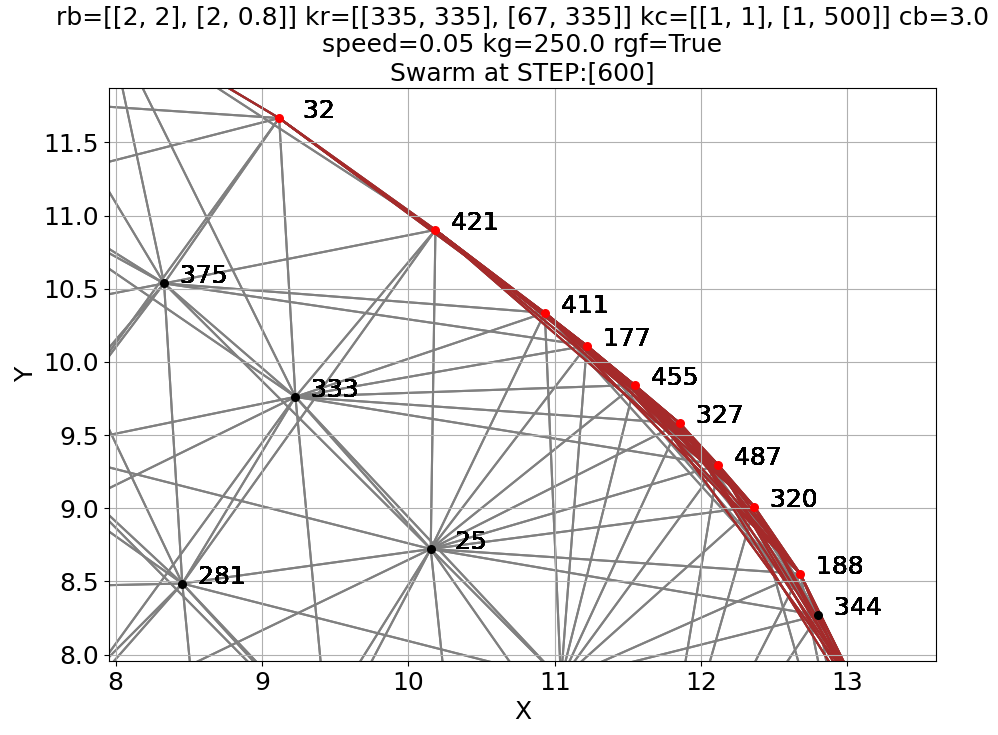
\includegraphics[width=8cm]{figures/perimeterCompress}
	\end{center}
	\caption{Swarm Example.\label{fig:swarmExample}}
\end{figure}
%\FloatBarrier

\subsection{Relationship-based swarm effects}

With the array form of $\rb, \kc, \kr$ we can now investigate the effect of pair-wise perimeter/internal relationships between agents on movement of the swarm and evolution of its structure and shape.

Using uniform arrays results in a simple cohesion/repulsion based swarm with all agents exhibiting the same properties similar to the original model discussed in \S~\ref{sec:basicModel}. However, modifying the arrays for specific relationships can induce emergent behaviours such as perimeter packing as discussed in \S~\ref{sec:perimCompress}.

\subsubsection{Cohesion model}~\\
When using Equation~\ref{eq:coh2} one array is used, $k_c$. This array is used to scale the cohesion vector generated between an agent pair which is proportional to their distance apart, which will be within $C$ as shown in Equation~\ref{eq:repulsion1a}. Consider the array shown in Equation~\ref{eq:kcexample1}.

\begin{equation}\label{eq:kcexample1}
	\kc = 
	\begin{bmatrix}
	1 & 1\\
	1 & 500
	\end{bmatrix}
\end{equation}

For a given agent pair their perimeter status will be calculated and applied to the array. If both agents are perimeter based then the value selected would be $k_c[P_b,P_{b'}] = 500$. If the agent pair were perimeter $\rightarrow$ non-perimeter then the value selected would be $k_c[P_b,P_{b'}] = 1$. This configuration would cause inter-perimeter agents to tend to move towards each other more strongly than any other relationship.\\~

\subsubsection{Repulsion model}~\\
When using Equation~\ref{eq:rep2} two arrays are used $\kr$ and $\rb$. $\kr$ is used to scale the resultant repulsion vector that is generated. $\rb$ is the radius of the repulsion field and is used to generate the proportion of the repulsion vector that is applied. Therefore consider the following two arrays (Eq's~\ref{eq:rexample1}~and~\ref{eq:krexample1}):

\begin{equation}\label{eq:rexample1}
	\rb = 
	\begin{bmatrix}
	2 & 2\\
	2 & 0.8
	\end{bmatrix}
\end{equation}

\begin{equation}\label{eq:krexample1}
	\kr = 
	\begin{bmatrix}
	335 & 335\\
	67 & 335
	\end{bmatrix}
\end{equation}

For a given agent pair their perimeter status will be calculated and applied to the arrays. If both agents are perimeter based then the values selected would be $\rb[P_b,P_{b'}] = 0.8$ and $\kr[P_b,P_{b'}] = 335$. If the agent pair were perimeter $\rightarrow$ non-perimeter then the values selected would be $\rb[P_b,P_{b'}] = 2$ and $\kr[P_b,P_{b'}] = 67$.\\

\section{Experimental results\label{sec:ExperimentalResults}}
The new modelling method allows for a highly configurable swarm. Each configuration has an impact on the swarm's structure. These changes are analysed using the inter-agent distances. The experimental results show the effects on the swarm in terms of inter-agent distances categorised by relationship. This section will cover four experiments and includes a baseline swarm for comparison.

\subsection{Distance metric}
Distance metrics are used by many researchers as a method of examining the structure of a swarm~\cite{BAFVM:06,BAF:06,elamvazhuthi2015optimal,VG:05,SW:03}. However, due to the new model allowing the field effects and magnitudes to be varied the distance metric will need to be adapted to analyse the agents involved in specific relationships rather than globally, therefore $S$ will be sub-divided into the three relationship categories of $S_i$, $S_p$, $S_{o}$. Where $S_i$ is the set of all internal\textrightarrow internal relationships, $S_p$ is the set of all perimeter\textrightarrow perimeter relationships and $S_{o}$ is the set of all internal\textrightarrow perimeter or perimeter\textrightarrow internal relationships. 
The metric is derived from the mean of a set of agent distances from its neighbours and the standard deviation of those agent sets. The mean is calculated as shown in equation~\ref{eq:SwarmStabilityDistance2} where $\mu_d(S)$ is the mean. The standard deviation is calculated as shown in equation~\ref{eq:SwarmStabilityDistance3} where $\sigma_d(S)$ is the standard deviation. The mean distance value can be compared to the repulsion field to identify if a swarm is optimally distributed in that the mean value should be as close to the repulsion field value as possible. The standard deviation identifies the overall differences in the distances which can be caused by the swarm agents oscillating. A standard deviation of $\sigma_d(S) = 0$ would indicate that all the agents are equally spaced.
\small
\begin{equation}
\label{eq:SwarmStabilityDistance2}
\mu_d(S) = \frac{\mathlarger{\sum_{b \in S}}~\mathlarger{\sum_{b' \in n_c(b)}}\magn{\vbb{b}{b'}}}{\mathlarger{\sum_{b \in S}\card{n_c(b)}}}
\end{equation}
\normalsize
\small
\begin{equation}
\label{eq:SwarmStabilityDistance3}
\sigma_d(S) = \sqrt{\frac{\mathlarger{\sum_{b \in S}}~\mathlarger{\sum_{b' \in n_c(b)}}\Big(\card{\vbb{b}{b'}} - \mu_d(S)\Big)^2}{\mathlarger{\sum_{b \in S}\card{n_c(b)}}}}
\end{equation}
\normalsize

The distance metric is therefore the distribution of a set of agents using both $\mu_d(S)$ and $\sigma_d(S)$. This can be written informally as:

\small
\begin{equation}
\label{eq:SwarmPotentialMagnitude}
\psi_d(S) = \mu_d(S)\pm \sigma_d(S)
\end{equation}
\normalsize

An example is shown in Figure~\ref{fig:tightPerimDistance}.

\subsection{Baseline Settings}
For all the experiments the parameters used to create the basic swarming effect are shown in table~\ref{tab:swarmingEffect}. Where $C$ is the cohesion field, $\kc$ is the cohesion weighting, $\rb$ is the repulsion field, $\kr$ is the repulsion weighting and $\kg$ is the weighting applied in the gap reduction algorithm discussed in~\cite{eliot2019void}. 

\begin{table}[H]
	\centering
	\tiny
	\begin{tabular}{|c|r|}
		\hline
		\rowcolor[HTML]{000000} 
		{\color[HTML]{FFFFFF} Swarming Variable} & {\color[HTML]{FFFFFF} Value} \\ \hline
		$C$ & \texttt{3.0} \\ \hline
		$k_c$ & \texttt{[[0.15,0.15][0.15,0.15]]}  \\ \hline
		$R$ & \texttt{[[2.0,2.0][2.0,2.0]]} \\ \hline
		$k_r$ & \texttt{[[50.0,50.0][50.0,50.0]]} \\ \hline
		$k_g$ & \texttt{0.0} \\ \hline
	\end{tabular}
	\caption{Swarming effect parameters}
	\label{tab:swarmingEffect}
\end{table}

\subsection{Baseline}
The baseline swarm consists of 400 agents which are distributed over and area of $20\times 20$ units ($-10\rightarrow+10$) as shown in Figure~\ref{fig:baselineSwarm1}. This is to simulate a randomised drop of agents into an area of interest. e.g. A field or airspace. The simulation is then allowed to stabilise. The resultant positions for the baseline swarm agents is shown in Figure~\ref{fig:baselineSwarm2}. 

\begin{figure}[H]
	\begin{center}
		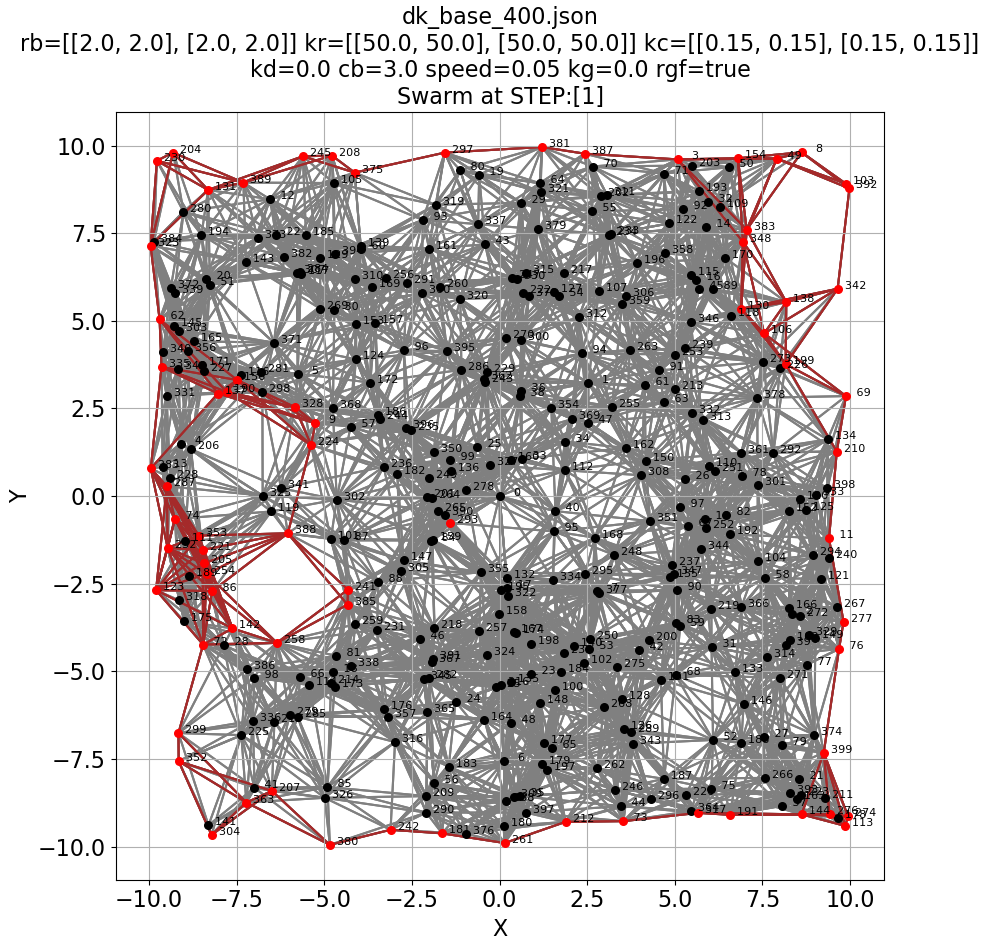
\includegraphics[width=1.0\linewidth]{figures/baseline1}
	\end{center}
	\caption{Baseline swarm. \label{fig:baselineSwarm1}}
\end{figure}
%\FloatBarrier

\begin{figure}[H]
	\begin{center}
		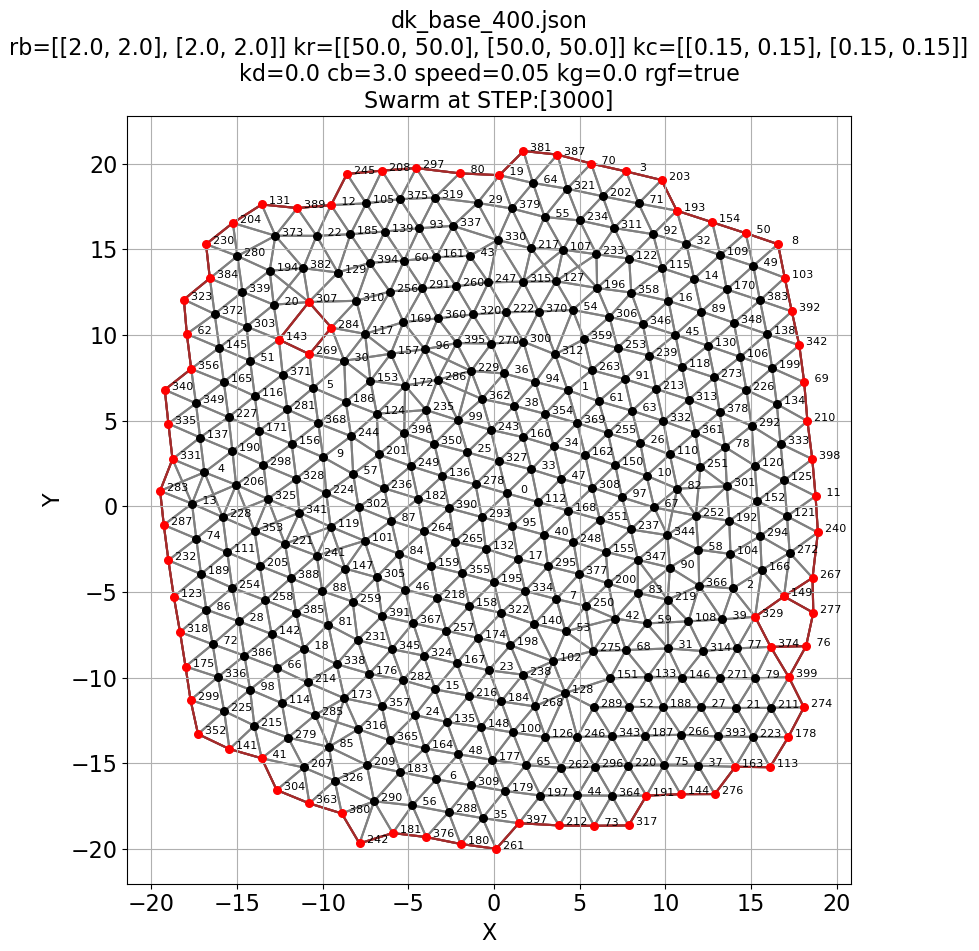
\includegraphics[width=1.0\linewidth]{figures/baseline2}
	\end{center}
	\caption{Baseline swarm. \label{fig:baselineSwarm2}}
\end{figure}
%\FloatBarrier

When the simulation is ran with no relationship differences i.e. all array values are equal. The distance graph shows the different agent relationships types split into $S_{i}$, $S_{p}$ and $S_{o}$ to allow a comparison with the new model. This state is used as the baseline for the experiments to measure the effects of changing the new arrays. The baseline configuration is equivalent to conventional swarming algorithms using single value potential fields.

The distance graph shows that perimeter\textrightarrow perimeter agents and internal\textrightarrow perimeter and perimeter \textrightarrow internal agents settle to a similar average distance of around 2.07 units and the internal agents settle to around 2.04 units. Given that the repulsion field is set to 2 units the swarm looks very stable and is able to form a lattice based structure that changes very little and has a small amount of jitter. Jitter is the slight variation in position that agents exhibit as they move to more optimum positions.

\begin{figure}[H]
	\begin{center}
		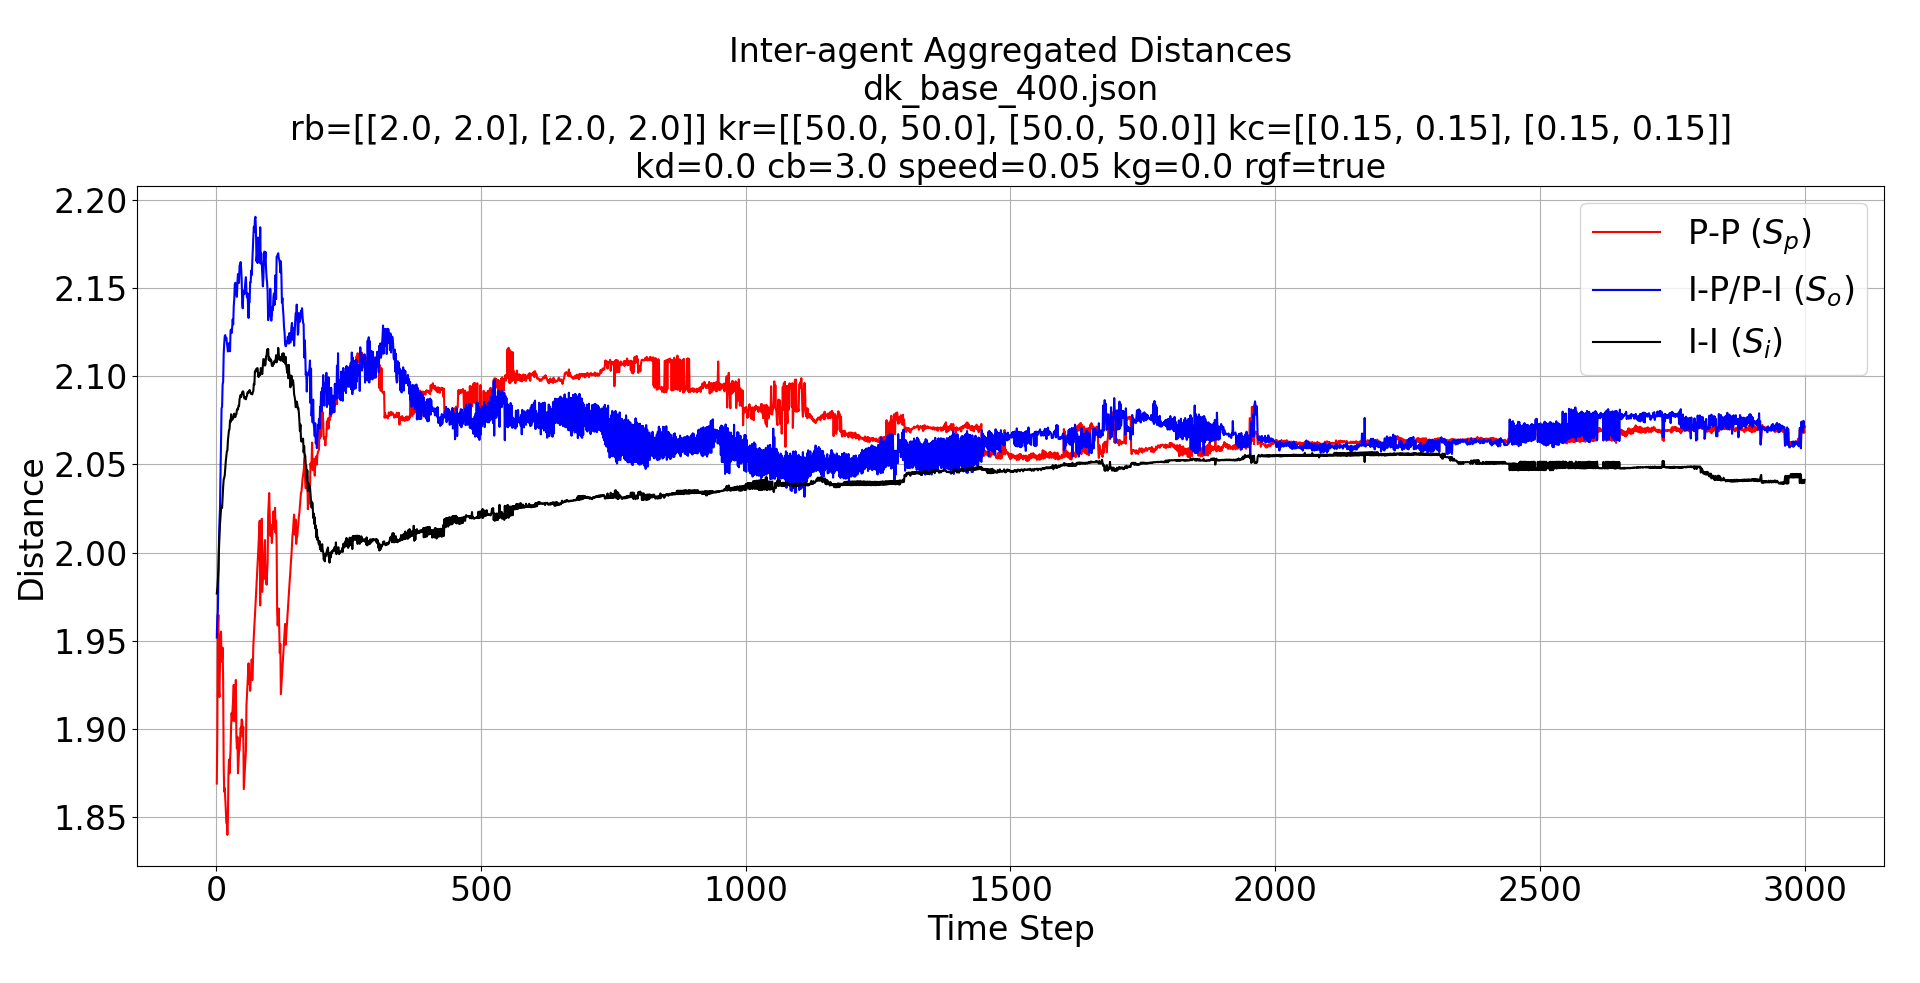
\includegraphics[width=1.0\linewidth]{figures/baselineDistance}
	\end{center}
	\caption{Baseline swarm (Distance). \label{fig:baselineDistance}}
\end{figure}
%\FloatBarrier

\subsubsection{Perimeter Packing}\label{sec:perimCompress}

The first experiment with the new model is to create a swarm that has a densely packed perimeter and by default exhibits a self-healing behaviour. This is achieved by modify the perimeter\textrightarrow perimeter agent relationship and the perimeter\textrightarrow non-perimeter/non-perimeter\textrightarrow perimeter relationship. The perimeter\textrightarrow perimeter agent repulsion field is reduced (Eq.~\ref{eq:rbexp1}) and the cohesion weighting is increased (Eq.~\ref{eq:kcexp1}), next the repulsion weighting of the perimeter\textrightarrow non-perimeter/non-perimeter\textrightarrow perimeter agents is reduced to allow the perimeter agents to pull closer together without the next layer of agents reducing the effect (Eq.~\ref{eq:krexp1}). 

\begin{equation}\label{eq:rbexp1}
\rb = 
\begin{bmatrix}
2.0 & 2.0\\
2.0 & 1.8
\end{bmatrix}
\end{equation}

\begin{equation}\label{eq:krexp1}
\kr = 
\begin{bmatrix}
50.0 & 10.0\\
50.0 & 50.0
\end{bmatrix}
\end{equation}

\begin{equation}\label{eq:kcexp1}
\kc = 
\begin{bmatrix}
0.15 & 0.15\\
0.15 & 75.0
\end{bmatrix}
\end{equation}

The resultant effect is that the perimeter agents are able to repel more internal neighbours before the aggregate repulsion prevents them moving closer as shown in figure~\ref{fig:tightPerim2}. As well as those changes a gap reduction effect is added ($\kg=100$). This effect includes closing the reflex angle ($\rgf=\mathsf{True}$) to smooth the perimeter inducing a compression effect on the perimeter. Using a high $\kg$ value creates a circular shaped swarm and stabilises the structure (Fig.~\ref{fig:tightPerim}).

\begin{figure}[H]
	\begin{center}
		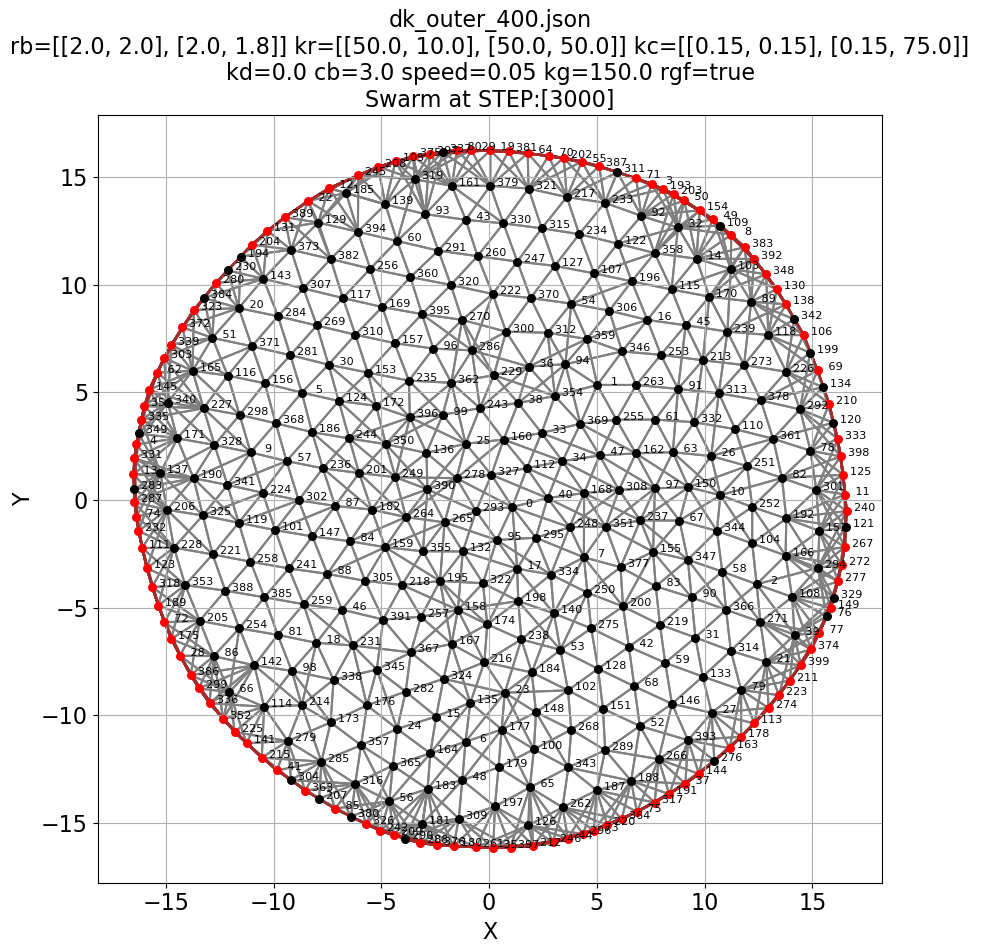
\includegraphics[width=1.0\linewidth]{figures/outer1}
	\end{center}
	\caption{Packed Perimeter 1. \label{fig:tightPerim}}
\end{figure}
%\FloatBarrier

\begin{figure}[H]
	\begin{center}
		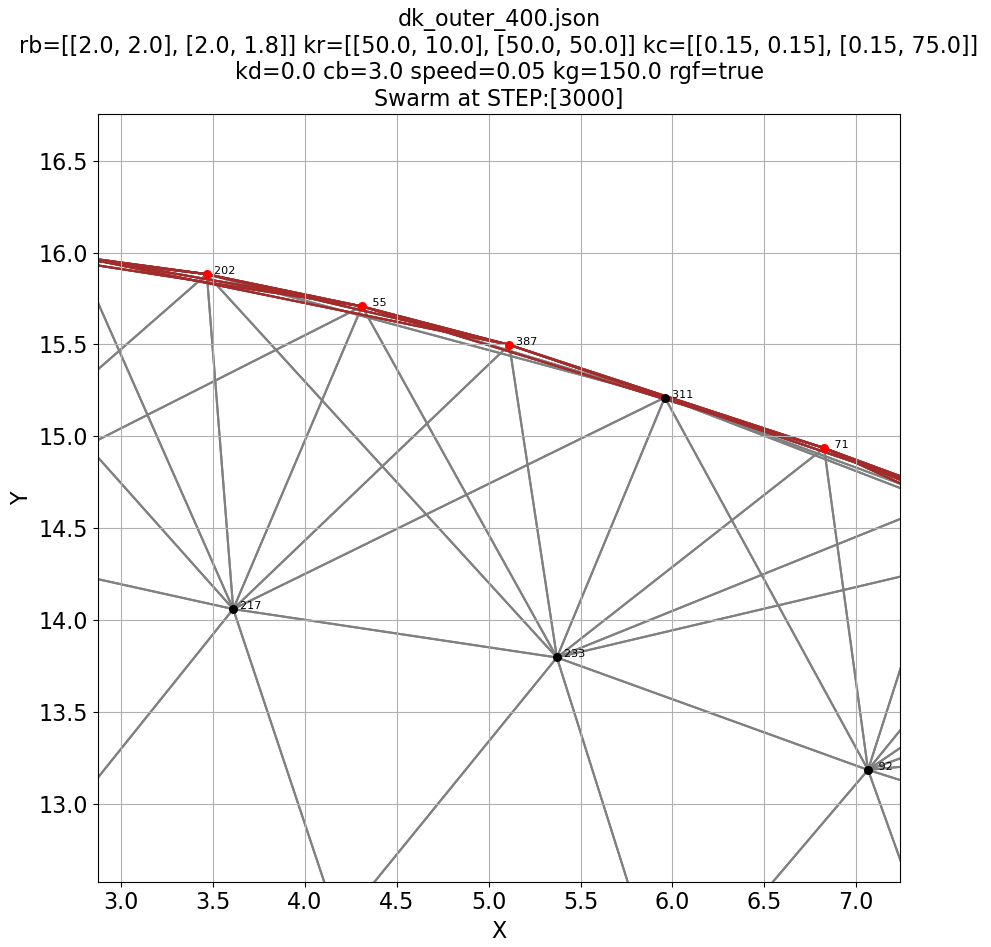
\includegraphics[width=1.0\linewidth]{figures/outer2}
	\end{center}
	\caption{Packed Perimeter 2. \label{fig:tightPerim2}}
\end{figure}
%\FloatBarrier

The effect of the parameters effects the swarm change the distribution of the agents. Figure~\ref{fig:tightPerimDistance} shows that the perimeter agents ($S_{p}$) are now closer together and that the distribution of the p\textrightarrow i and i\textrightarrow p agents ($S_{i}$, $S_{o}$) are now of a similar distance apart which allows the internal agents to form a regular hexagonal lattice.

\begin{figure}[H]
	\begin{center}
		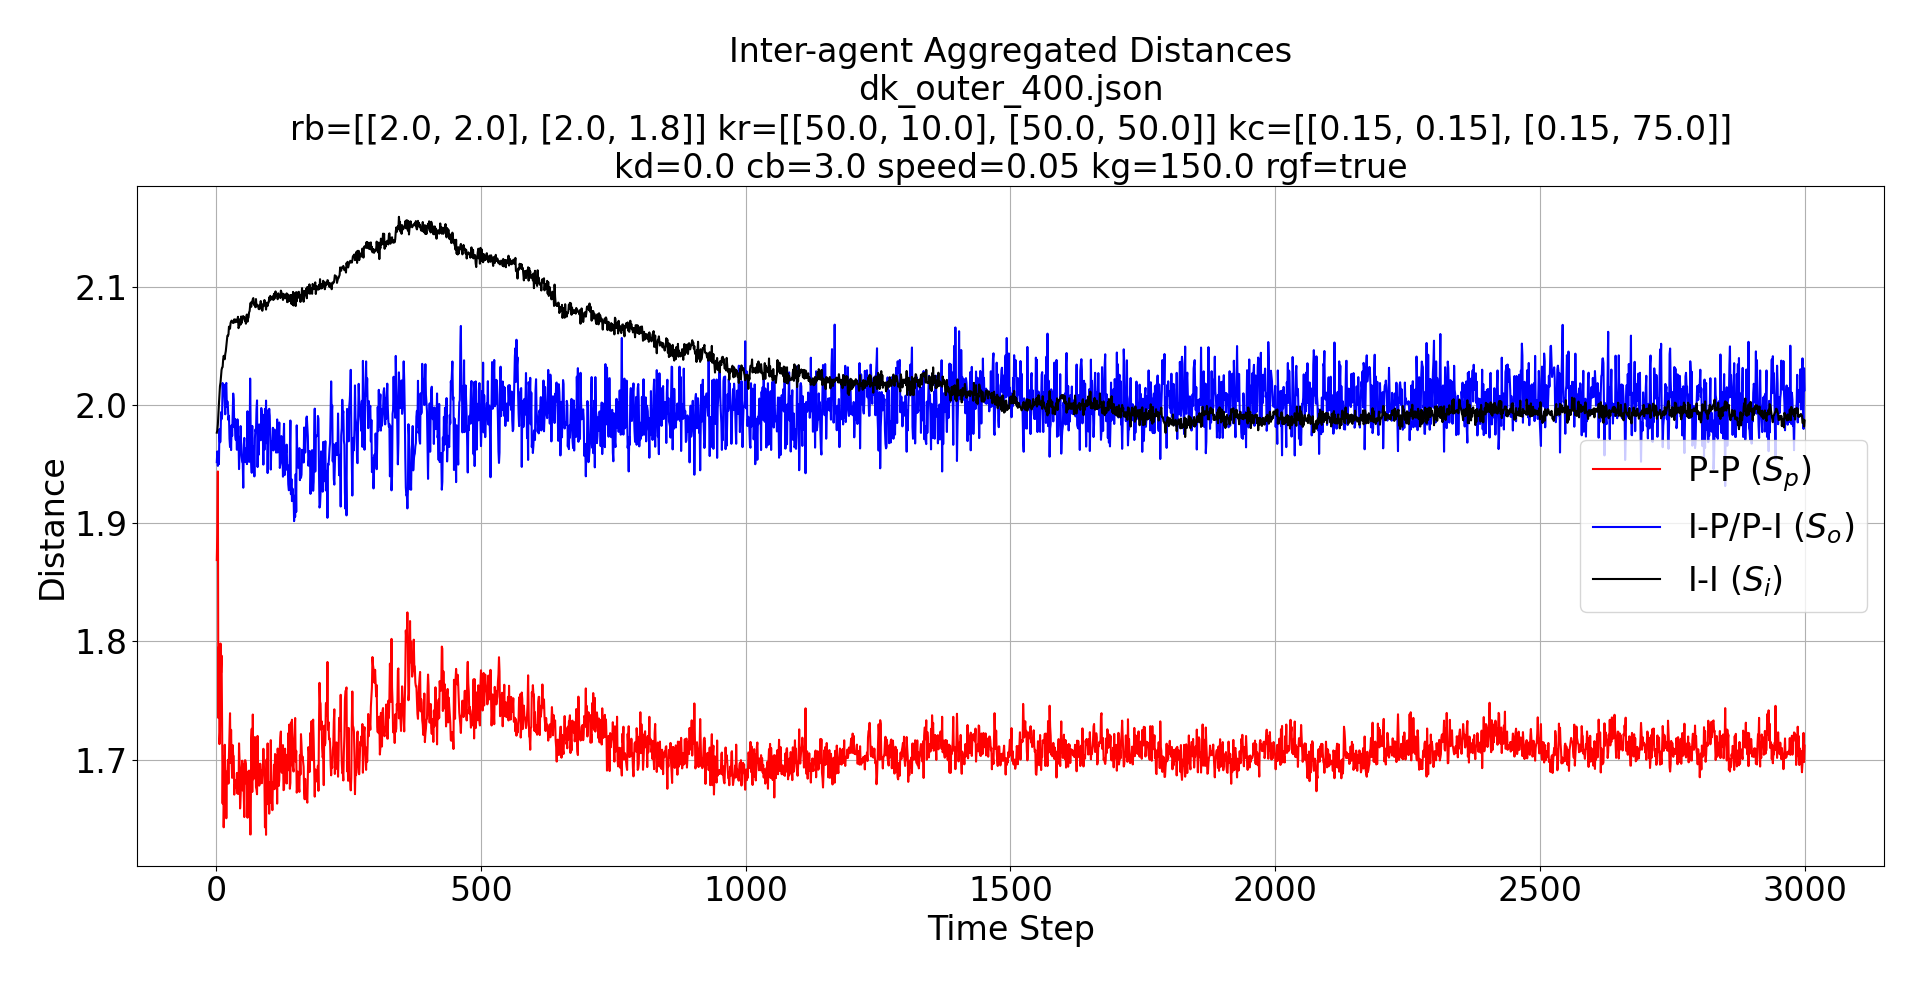
\includegraphics[width=1.0\linewidth]{figures/outerDistance}
	\end{center}
	\caption{Packed Perimeter (Distance). \label{fig:tightPerimDistance}}
\end{figure}
%\FloatBarrier

\subsubsection{Perimeter Expansion}
The basis of this experiment is to use the new model to generate a swarm that allows a swarm to expand from a condensed deployment state and increase the distance between perimeter-based agents while maintaining a dense core. This would be useful when a swarm is moving into an area that could disable or harm agents to reduce the number of agents and limit the number of agents that would be lost from the swarm. This effect has the added benefit in that the swarm will also exhibit a self-healing property due to the internal compression.

The parameters shown in equation~\ref{eq:rbexp2},~\ref{eq:krexp2}~and~\ref{eq:kcexp2} are designed to create a distancing between perimeter\textrightarrow perimeter agents by holding them steady with an increased cohesion weighting (150.0) and at the same time creating a high degree of repulsion between non-perimeter\textrightarrow perimeter agents (1000.0) i.e. the non-perimeter agents repel the perimeter agents as shown in figure~\ref{fig:perimExpand2}.

\begin{equation}\label{eq:rbexp2}
\rb = 
\begin{bmatrix}
2.0 & 2.0\\
2.0 & 2.0
\end{bmatrix}
\end{equation}

\begin{equation}\label{eq:krexp2}
\kr = 
\begin{bmatrix}
50.0 & 1000.0\\
50.0 & 50.0
\end{bmatrix}
\end{equation}

\begin{equation}\label{eq:kcexp2}
\kc = 
\begin{bmatrix}
0.15 & 0.15\\
0.15 & 15.0
\end{bmatrix}
\end{equation}

As well as those changes a gap reduction effect is added ($\kg=50$). This effects, which includes closing the reflex angle ($\rgf=\mathsf{True}$), has the effect of `smoothing' the perimeter to create a circular shape as shown in figure~\ref{fig:perimExpand1}.

\begin{figure}[H]
	\begin{center}
		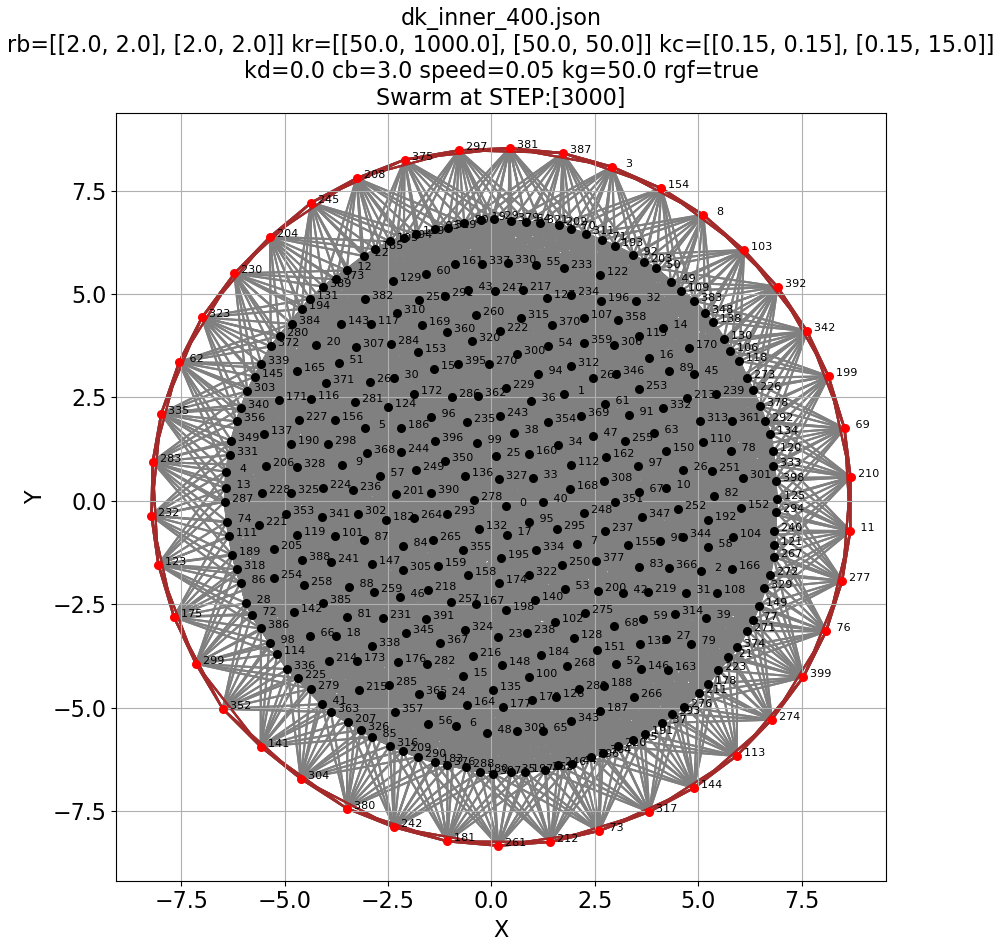
\includegraphics[width=1.0\linewidth]{figures/inner1}
	\end{center}
	\caption{Perimeter Expanded 1. \label{fig:perimExpand1}}
\end{figure}
%\FloatBarrier

\begin{figure}[H]
	\begin{center}
		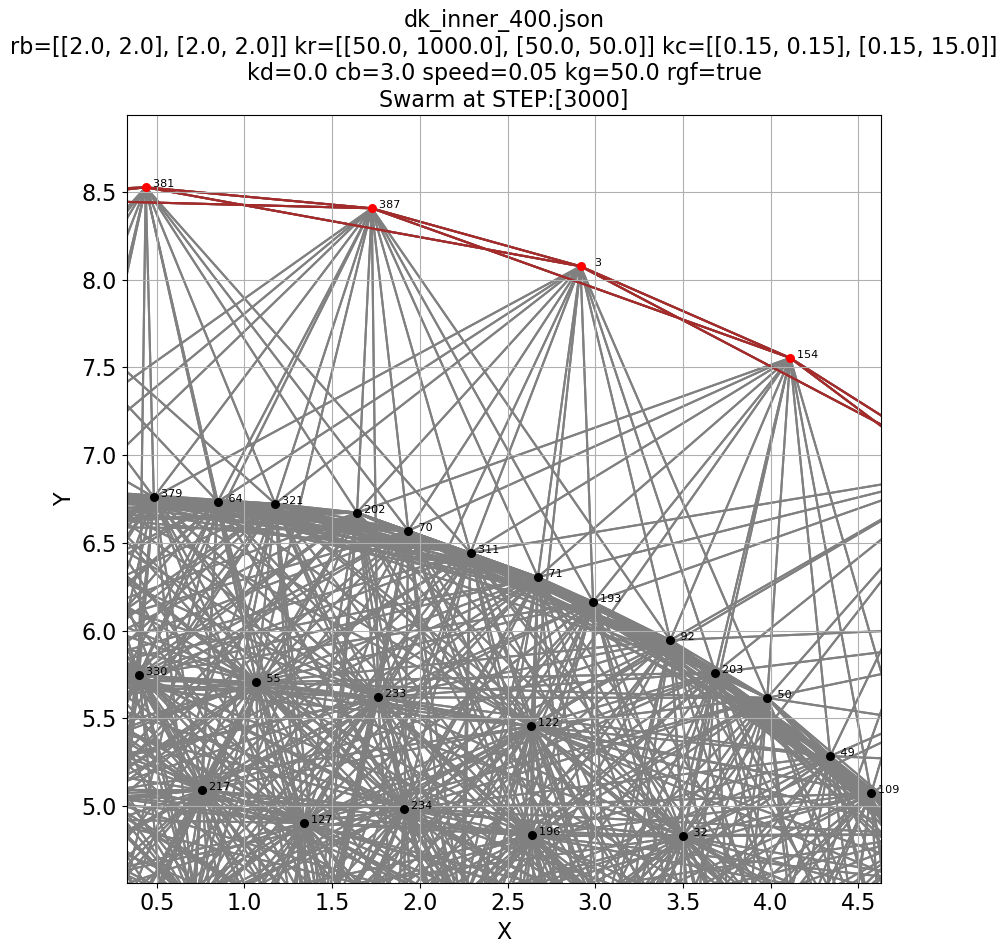
\includegraphics[width=1.0\linewidth]{figures/inner2}
	\end{center}
	\caption{Perimeter Expanded 2. \label{fig:perimExpand2}}
\end{figure}
%\FloatBarrier

The effect on the inter-agent distances is shown in figure~\ref{fig:perimExpandDistance}. It shows that the perimeter agents ($S_p$) are well distributed and almost on the limits of the repulsion field ($\rb$). However, $s_i$ has a high degree of modality indicated by the large $\psi_p$ of the agents and $S_o$ shows that the internal\textrightarrow internal agents are, on average, holding steady well beyond the repulsion field, again due to the modality.

\begin{figure}[H]
	\begin{center}
		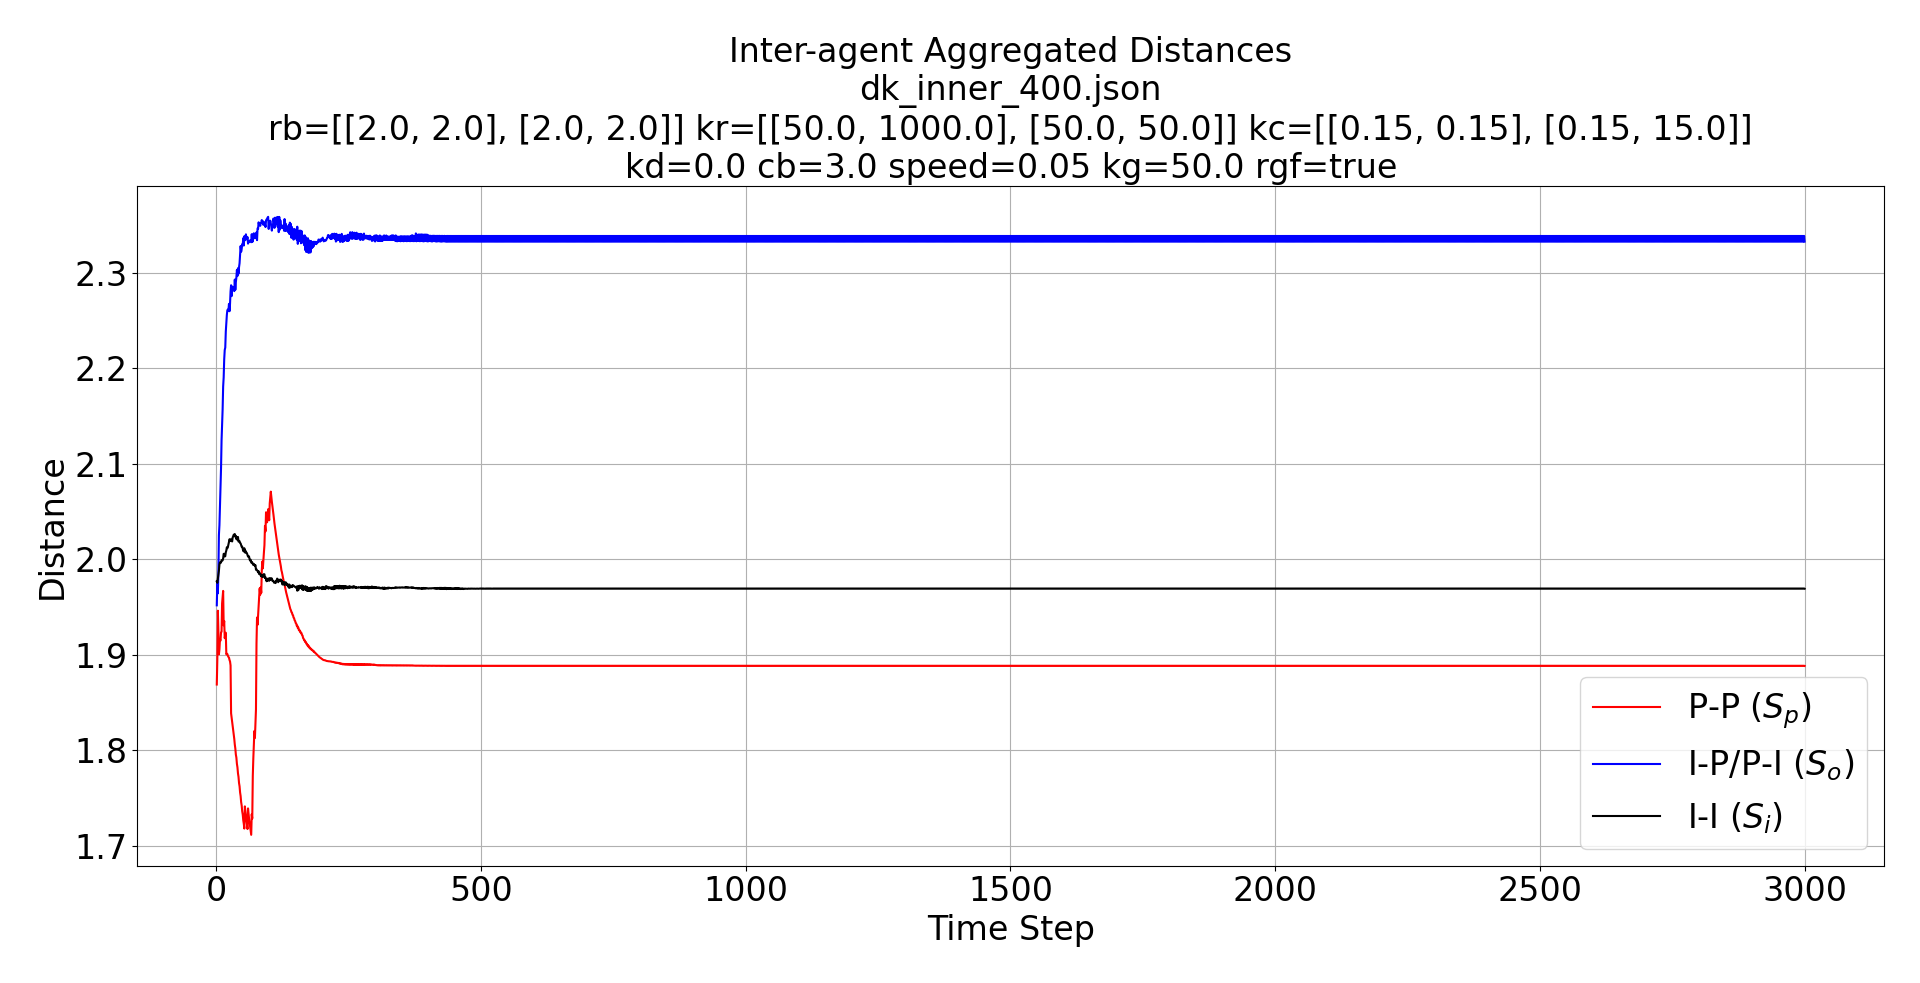
\includegraphics[width=1.0\linewidth]{figures/innerDistance}
	\end{center}
	\caption{Perimeter Expanded (Distance). \label{fig:perimExpandDistance}}
\end{figure}
%\FloatBarrier

Examining the distances more closely it can be seen that the standard deviation is high which indicates that the swarm is multi-model. A multi-model swarm is created when agents are able to see multiple agents within the cohesion field beyond the regular hexagonal distribution. The perimeter\textrightarrow perimeter distribution (Fig.~\ref{fig:perimExpandDistancePP}) is less model than the perimeter\textrightarrow non-perimeter non-perimeter\textrightarrow perimeter group (Fig.~\ref{fig:perimExpandDistanceIPPI}) and the internal agents are highly model (Fig.~\ref{fig:perimExpandDistanceII}).

\begin{figure}[H]
	\begin{center}
		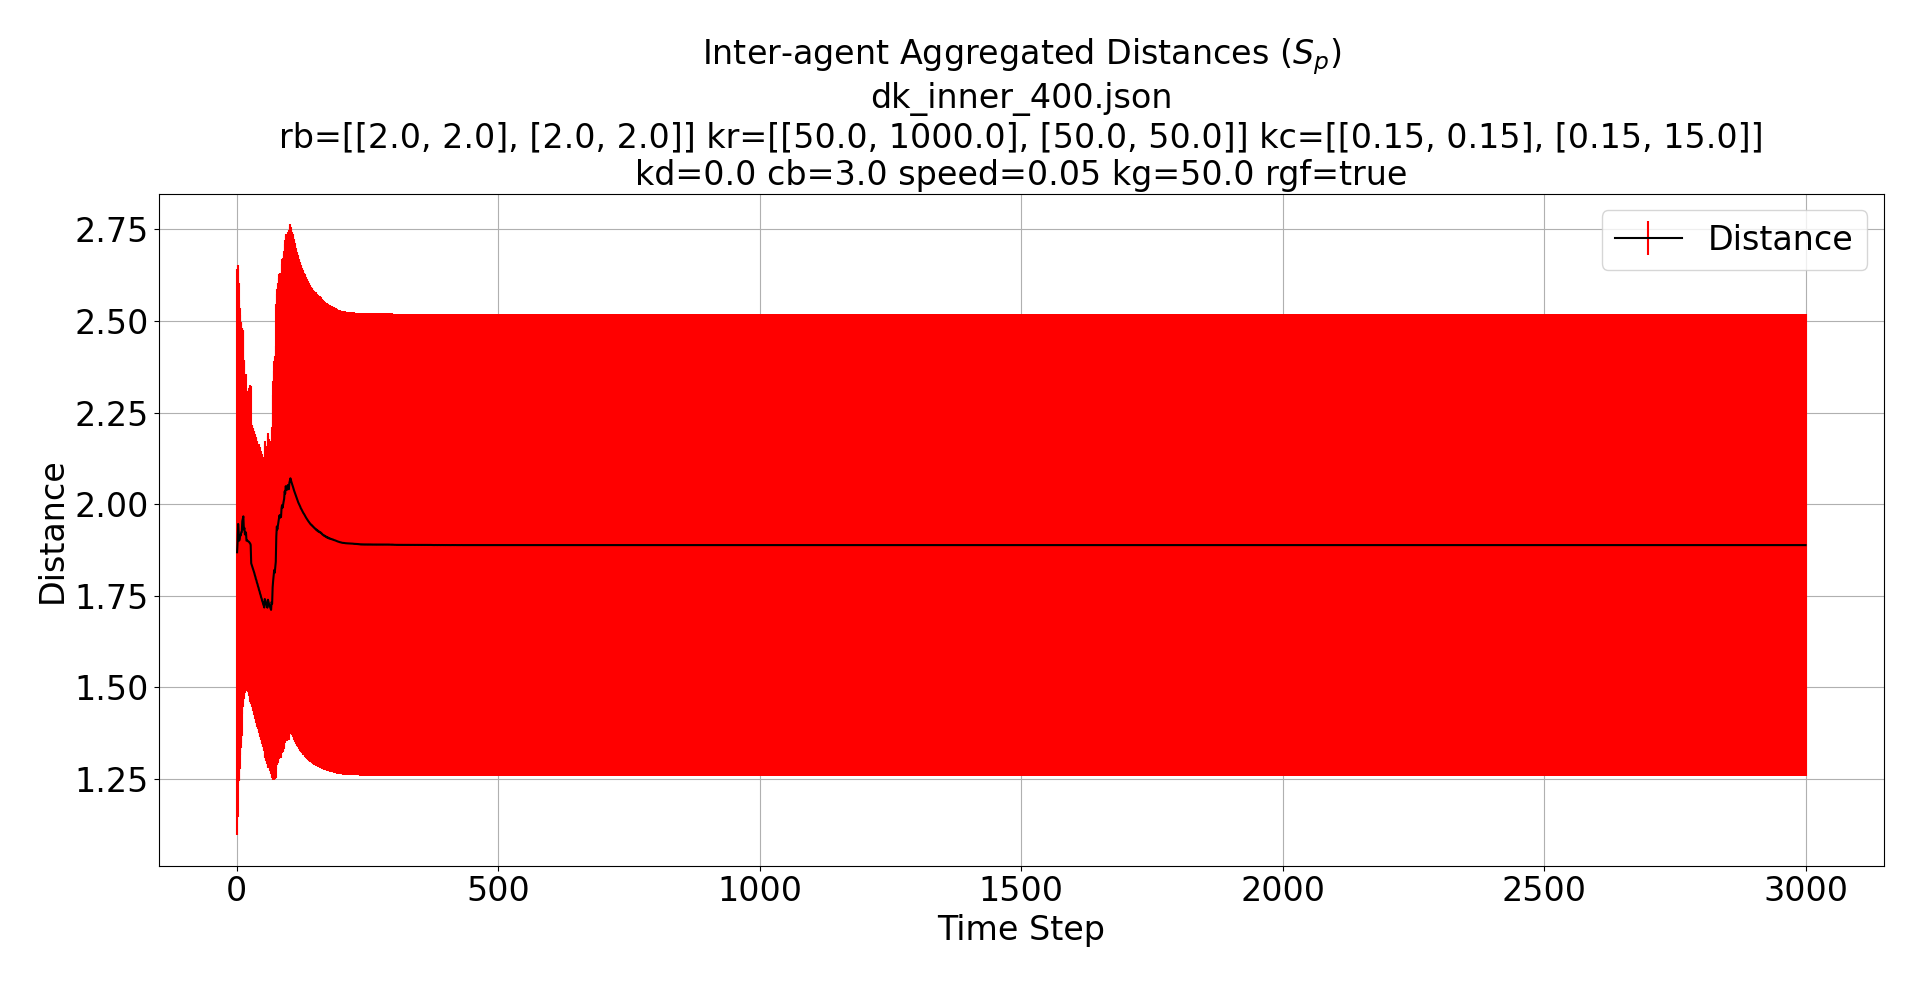
\includegraphics[width=1.0\linewidth]{figures/innerDistancePP}
	\end{center}
	\caption{Perimeter Expanded PP (Distance). \label{fig:perimExpandDistancePP}}
\end{figure}
%\FloatBarrier

\begin{figure}[H]
	\begin{center}
		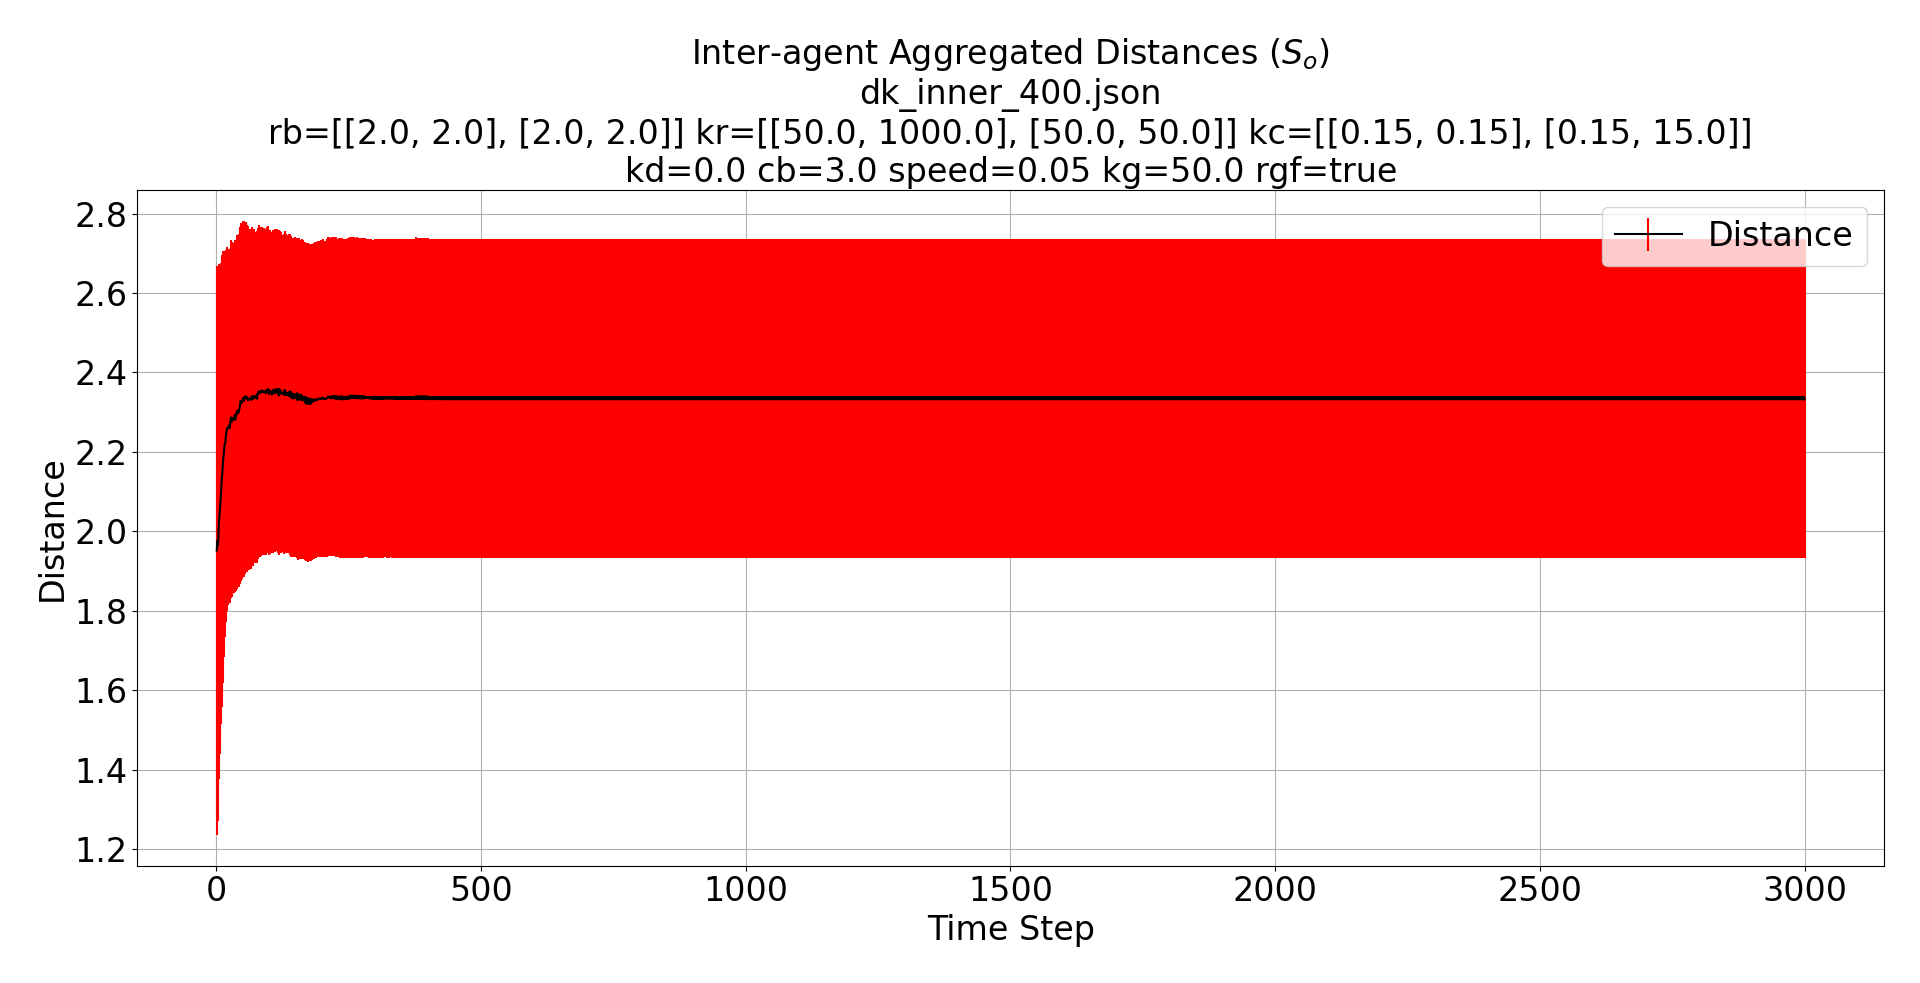
\includegraphics[width=1.0\linewidth]{figures/innerDistanceIPPI}
	\end{center}
	\caption{Perimeter Expanded IPPI (Distance). \label{fig:perimExpandDistanceIPPI}}
\end{figure}
%\FloatBarrier

\begin{figure}[H]
	\begin{center}
		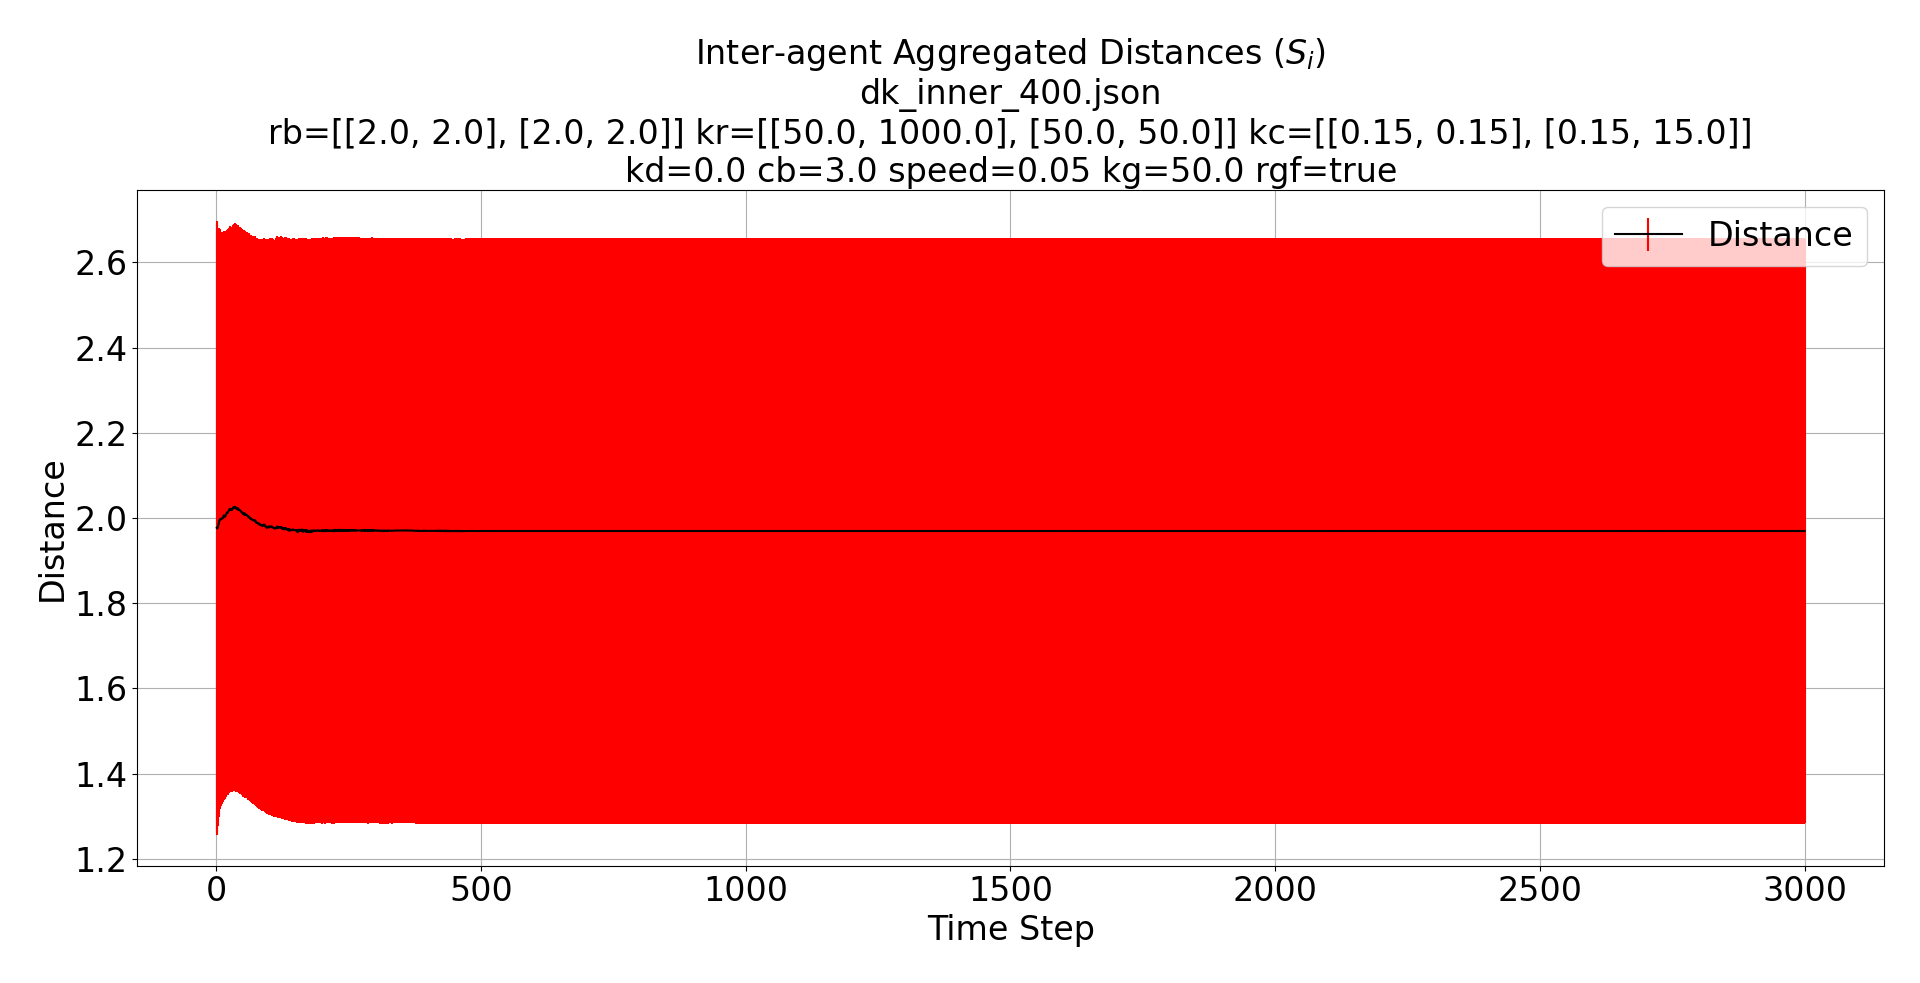
\includegraphics[width=1.0\linewidth]{figures/innerDistanceII}
	\end{center}
	\caption{Perimeter Expanded II (Distance). \label{fig:perimExpandDistanceII}}
\end{figure}
%\FloatBarrier

\subsubsection{$\kg$ gap reduction}

The aim of this experiment is to show the effect of using the gap reduction mechanism on it own to see the part it plays in the new model. The reduction method is an extension of the method used by Eliot et al.~\cite{eliot2018metric}. The mechanics are the same but the reflex angle can be identified as a gap to add additional control to a perimeters structure. The $\rb$, $\kr$ and $\kc$ values are all set to the baseline and $kg=100$.

Figure~\ref{fig:gap1} shows the final (step 3000) of the simulation. It shows that the swarm has expanded from its initial state and due to the effects of $\kg$ the swarms has formed a compressed circular swarm.

\begin{figure}[H]
	\begin{center}
		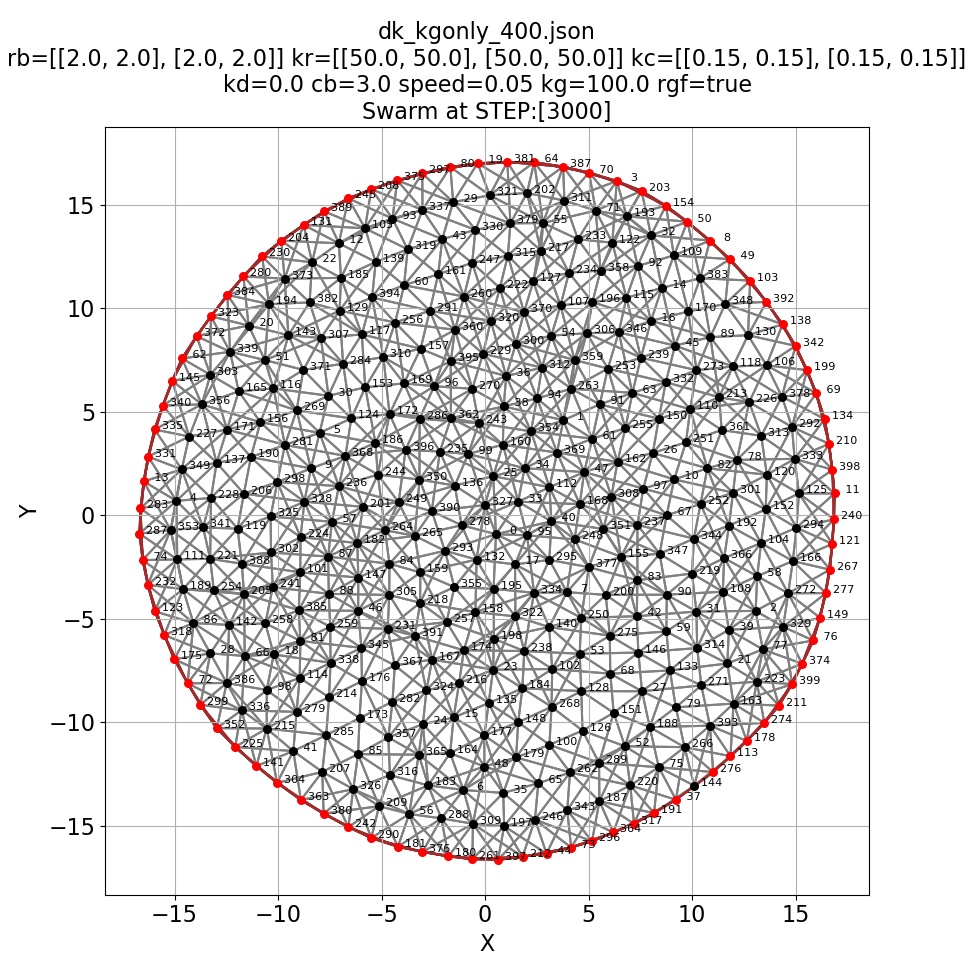
\includegraphics[width=1.0\linewidth]{figures/gap1}
	\end{center}
	\caption{Gap reduction 1. \label{fig:gap1}}
\end{figure}
%\FloatBarrier

Figure~\ref{fig:gap2} shows that although the swarm structure has been brought together as a circular swarm the perimeter is only slightly compressed. This is due to the reflex angle `pulling' the agents in but the repulsion between the perimeter agents prevents them from moving more closely together. 

\begin{figure}[H]
	\begin{center}
		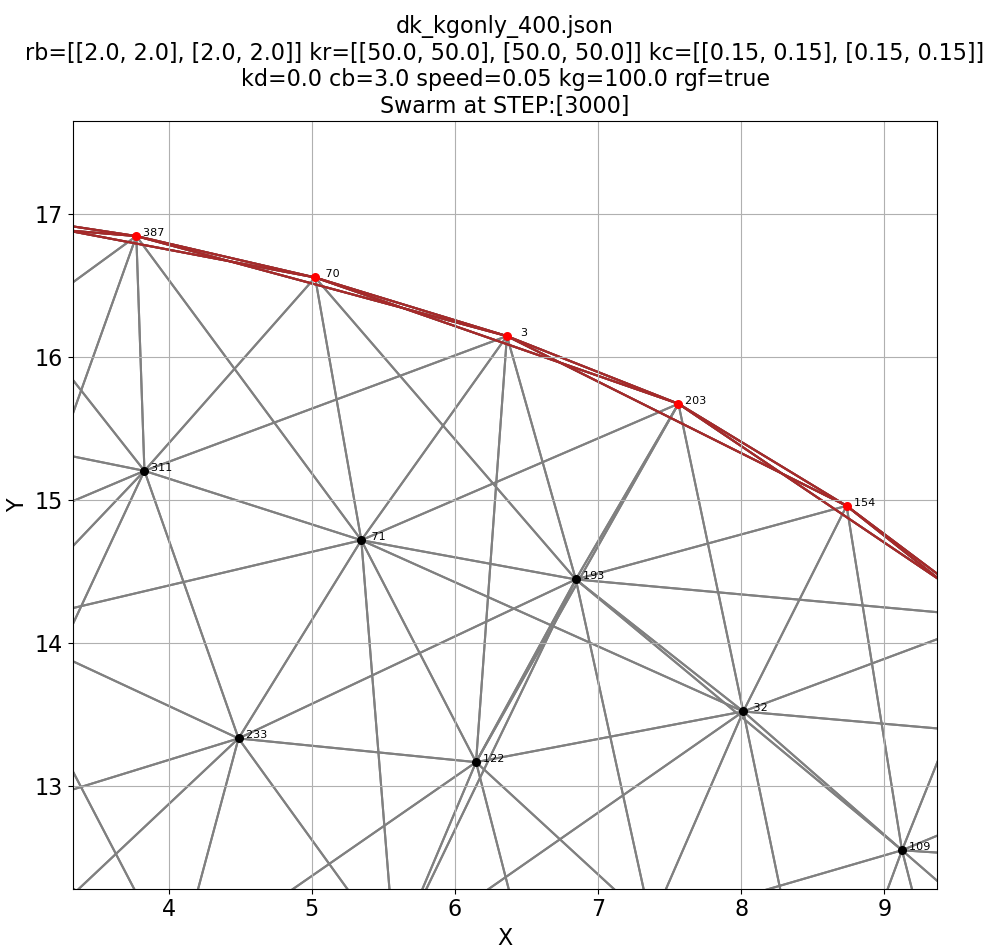
\includegraphics[width=1.0\linewidth]{figures/gap2}
	\end{center}
	\caption{Gap reduction 2. \label{fig:gap2}}
\end{figure}
%\FloatBarrier

Figure~\ref{fig:gapDistance} shows that the swarm perimeter is slightly compressed as the distance is just below the repulsion field, where as the internal and perimeter\textrightarrow non-perimeter/non-perimeter\textrightarrow perimeter agents have an average distance that is beyond the repulsion field which indicated a multi-model/compressed arrangement with the internal\textrightarrow internal agents being slightly less compressed.

\begin{figure}[H]
	\begin{center}
		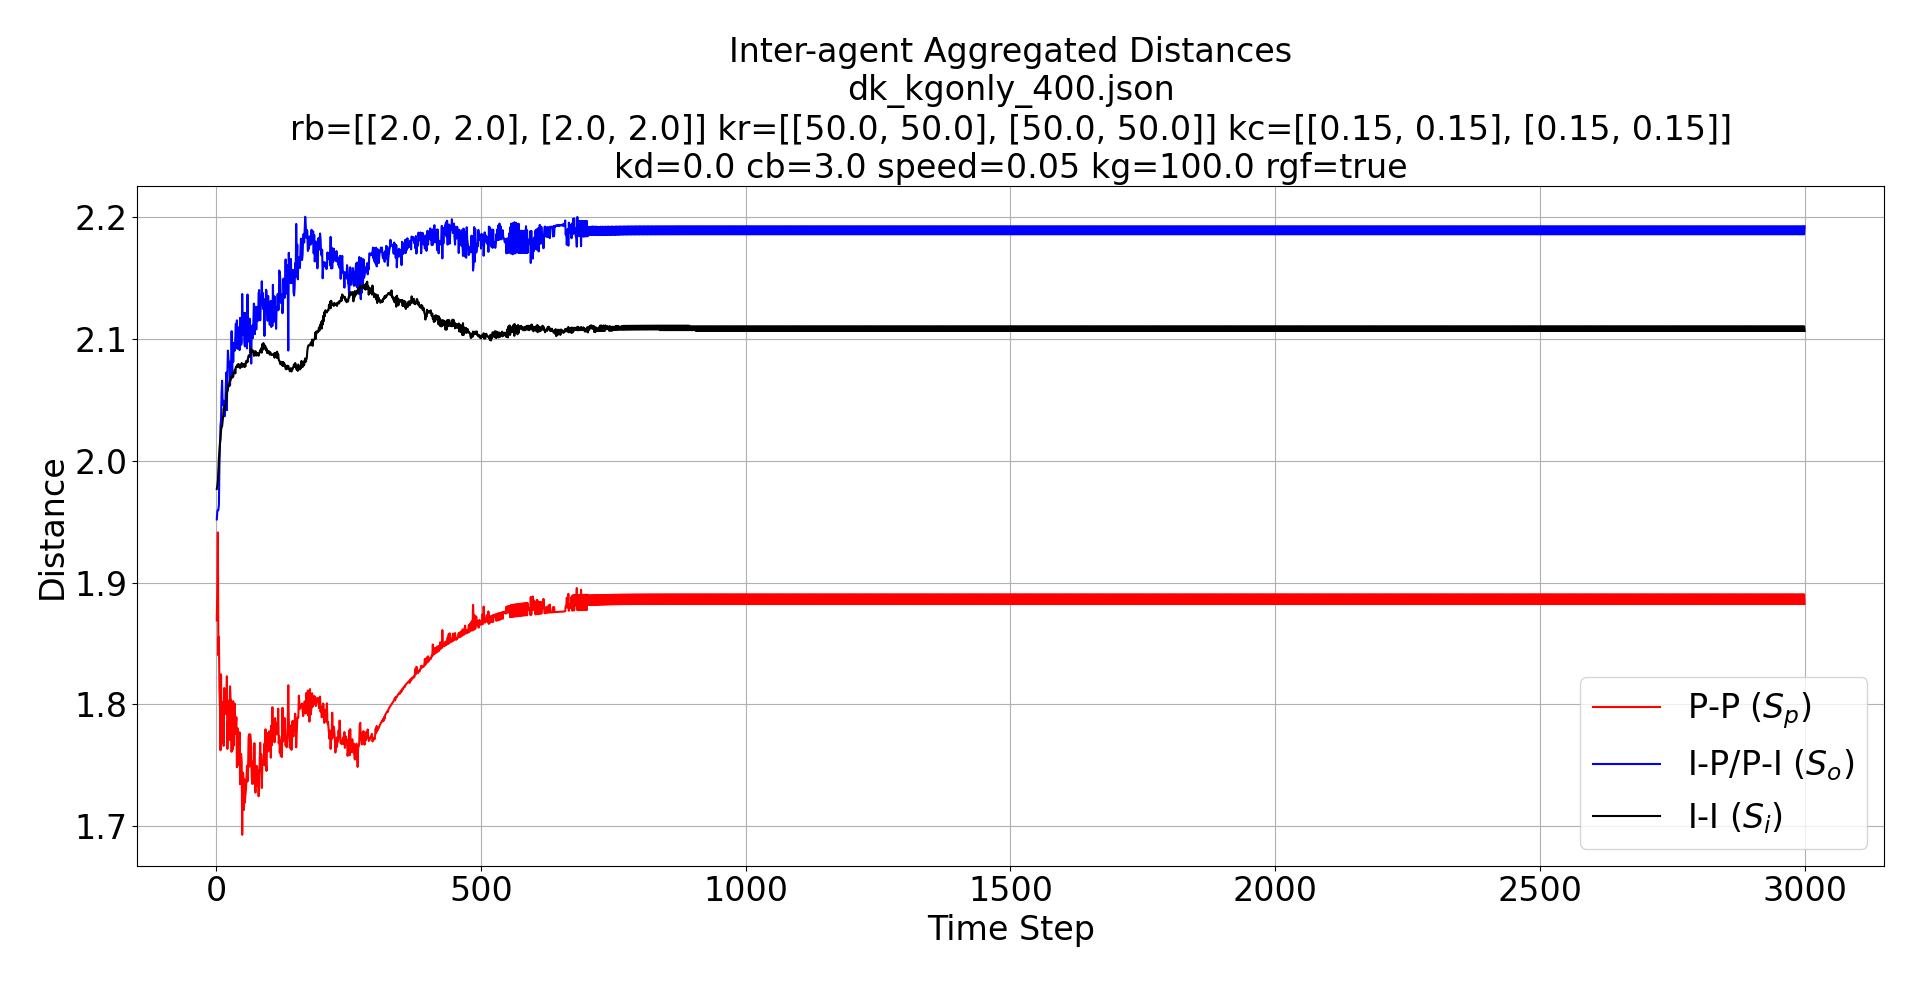
\includegraphics[width=1.0\linewidth]{figures/gapDistance}
	\end{center}
	\caption{Gap Distance\label{fig:gapDistance}}
\end{figure}
%\FloatBarrier

\subsubsection{Void Removal and Perimeter Packing}

In this experiment the swarm consists of 400 agents which are distributed over and area of roughly $25\times 25$ units as shown in Figure~\ref{fig:voidPerim1} and consists of agents that are relatively evenly spaced with a large void in the centre of the swarm. 

\begin{figure}[H]
	\begin{center}
		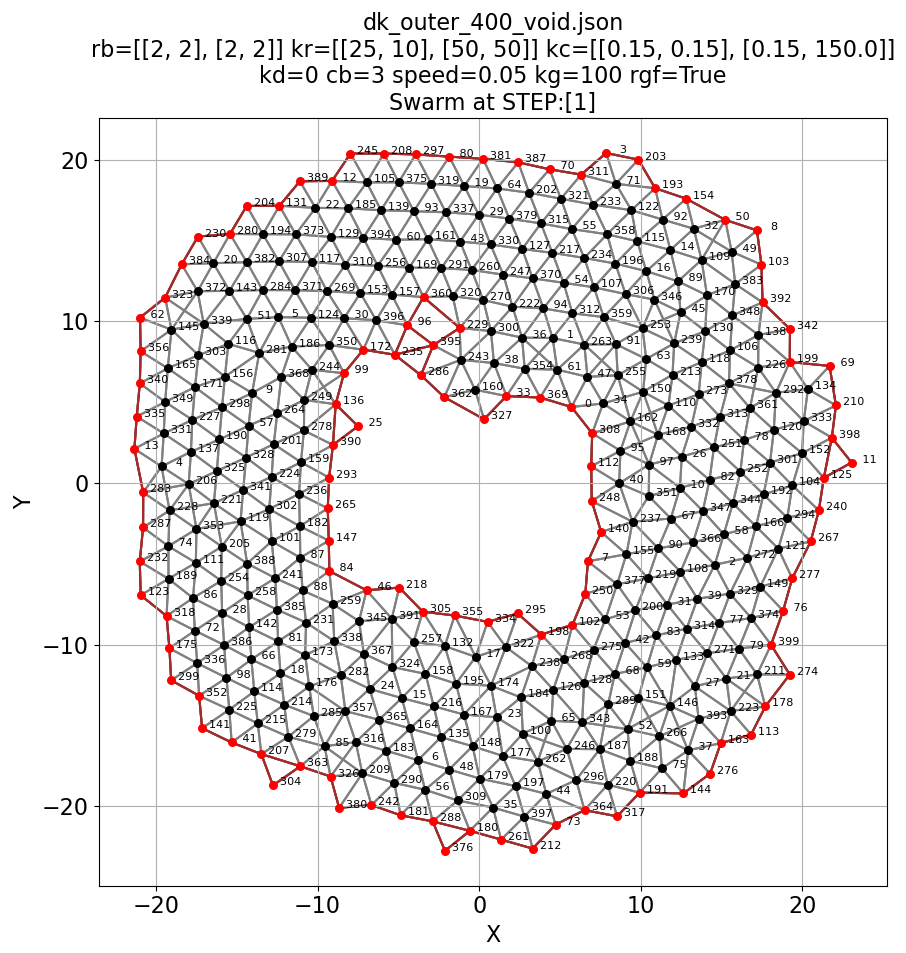
\includegraphics[width=1.0\linewidth]{figures/voidPerim1}
	\end{center}
	\caption{Void removal and Perimeter Packing 1\label{fig:voidPerim1}}
\end{figure}
%\FloatBarrier

The basis for this experiment is to show that the new algorithm can be tuned to heal the swarm by removing the void and also create a packed perimeter formation. The parameters used to create the effect are based upon the baseline swarm parameters with the changes to $\rb$, $\kr$ and $\kc$ shown in equations~\ref{eq:voidPerim1},~\ref{eq:voidPerim2}~and~\ref{eq:voidPerim3}.

\begin{equation}\label{eq:voidPerim1}
	\rb = 
	\begin{bmatrix}
	2.0 & 2.0\\
	2.0 & 2.0
	\end{bmatrix}
\end{equation}
	
\begin{equation}\label{eq:voidPerim2}
	\kr = 
	\begin{bmatrix}
	25.0 & 10.0\\
	50.0 & 50.0
	\end{bmatrix}
\end{equation}

\begin{equation}\label{eq:voidPerim3}
	\kc = 
	\begin{bmatrix}
	0.15 & 0.15\\
	0.15 & 150.0 
	\end{bmatrix}
\end{equation}

Figure~\ref{fig:voidPerim2} shows the resultant swarm formation after 3000 epochs. It shows the void has been removed and the perimeter of the swarm is tightly packed. This has been achieved by reducing the $\kr$ value of the non-perimeter\textrightarrow non-perimeter agents ($\kr=25$) allowing the internal structure of the swarm to be compressed by the perimeter. At the same time the non-perimeter\textrightarrow perimeter repulsion has be reduced further $\kr=10$ to allow the perimeter agents to move more closely before the aggregate effect of the next layer of agents impacts upon the reduced perimeter distances. The $\kc$ settings for perimeter\textrightarrow perimeter agents is increased ($kg=150.0$) to pull the perimeter agents together.

\begin{figure}[H]
	\begin{center}
		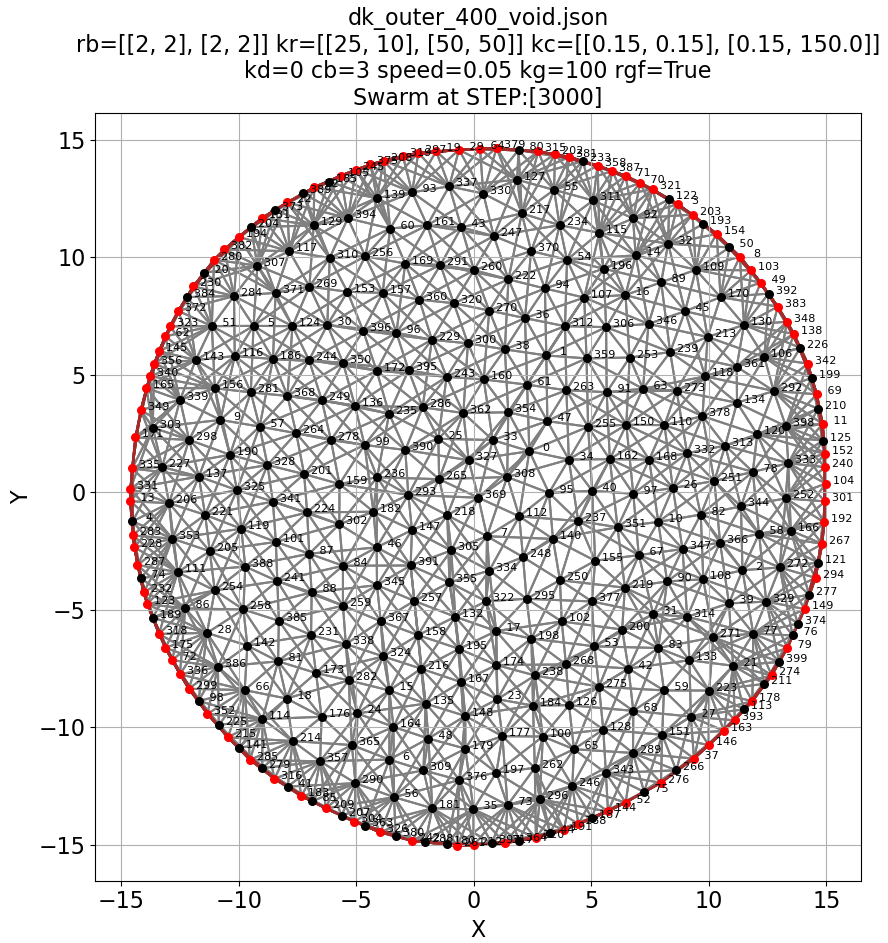
\includegraphics[width=1.0\linewidth]{figures/voidPerim2}
	\end{center}
	\caption{Void removal and Perimeter Packing 2\label{fig:voidPerim2}}
\end{figure}
%\FloatBarrier

Figure~\ref{fig:voidPerimDistance} shows that the perimeter agents are closer together, the base repulsion field is set to 2 nits and the agents are ~1.7 units apart. The internals of the swarm are highly model and therefore the distance is averaging beyond the repulsion field and the layer below the perimeter has more a lower average use to the increased repulsion holding the agents.

\begin{figure}[H]
	\begin{center}
		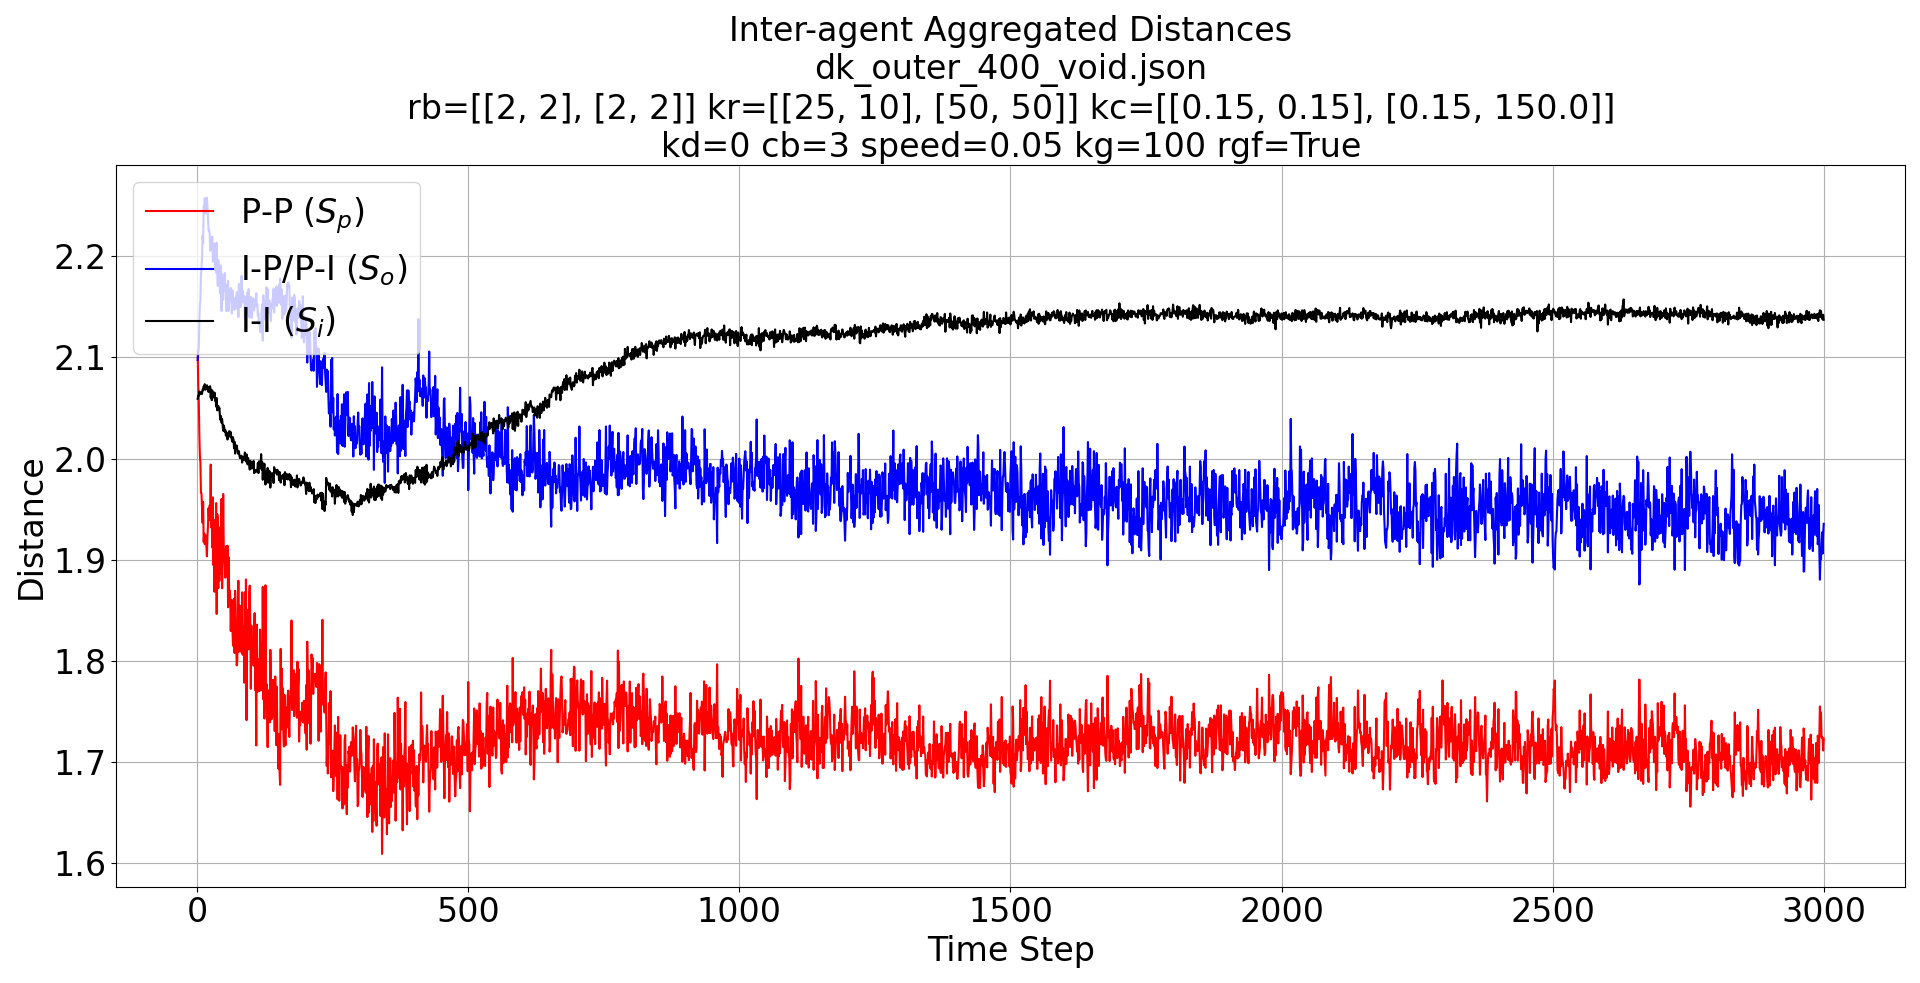
\includegraphics[width=1.0\linewidth]{figures/voidPerimDistance}
	\end{center}
	\caption{Void and Perimeter Packing (Distance)\label{fig:voidPerimDistance}}
\end{figure}
%\FloatBarrier

\section{Conclusions and future work}\label{conclusions}
From the initial simulations it is possible to show that the technique is able to successfully restructure swarms into usable configurations based upon the requirements of 4 distinct relationships. Also, by adjusting the gap reduction vector $\kg$ to not use the reflex angles it is possible to allow the perimeter agents to circulate around areas that form naturally on the perimeter. This requires more analysis to fully realise its potential and application. The effect can be seem in the video at \url{https://youtu.be/E4Q4hk4KrWA}. Additionally it is possible to remove voids and therefore surround obstacles. The metric show that the algorithm does have an impact on swarm stability to exhibit these new features but the impact is consistent throughout the swarms lifetime as it migrates into different structures.

Going forward the new model will be examined based upon alternative magnitude based metrics and the introduction of a directional bias along with obstacle avoidance/surrounding. Initial testing shows that the model holds up well including the improvement in self-healing as demonstrated in figure~\ref{fig:packedSelfHealing} which shows an obstacle being introduced and removed in a packed perimeter swarm. Figure~\ref{fig:future8} shows the impact the obstacle introduction has upon the inter-agent distances.

\begin{figure*}[!ht]
  \begin{center}
    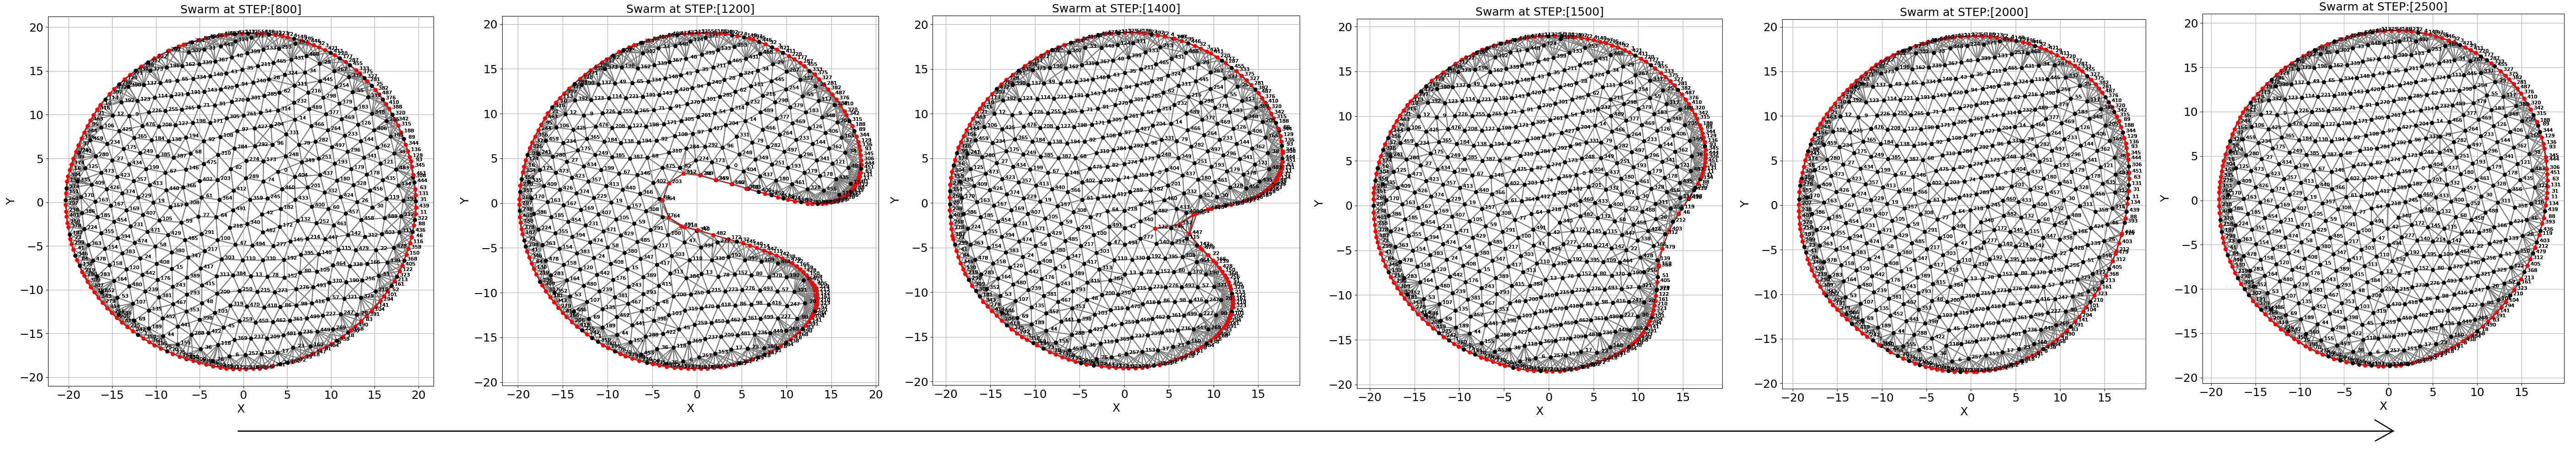
\includegraphics[width=17.6cm]{figures/FutureTime}
  \end{center}
  \caption{Simulation of a packed perimeter demonstrating self-healing properties over time\label{fig:packedSelfHealing}}
\end{figure*}

\begin{figure}[H]
	\begin{center}
		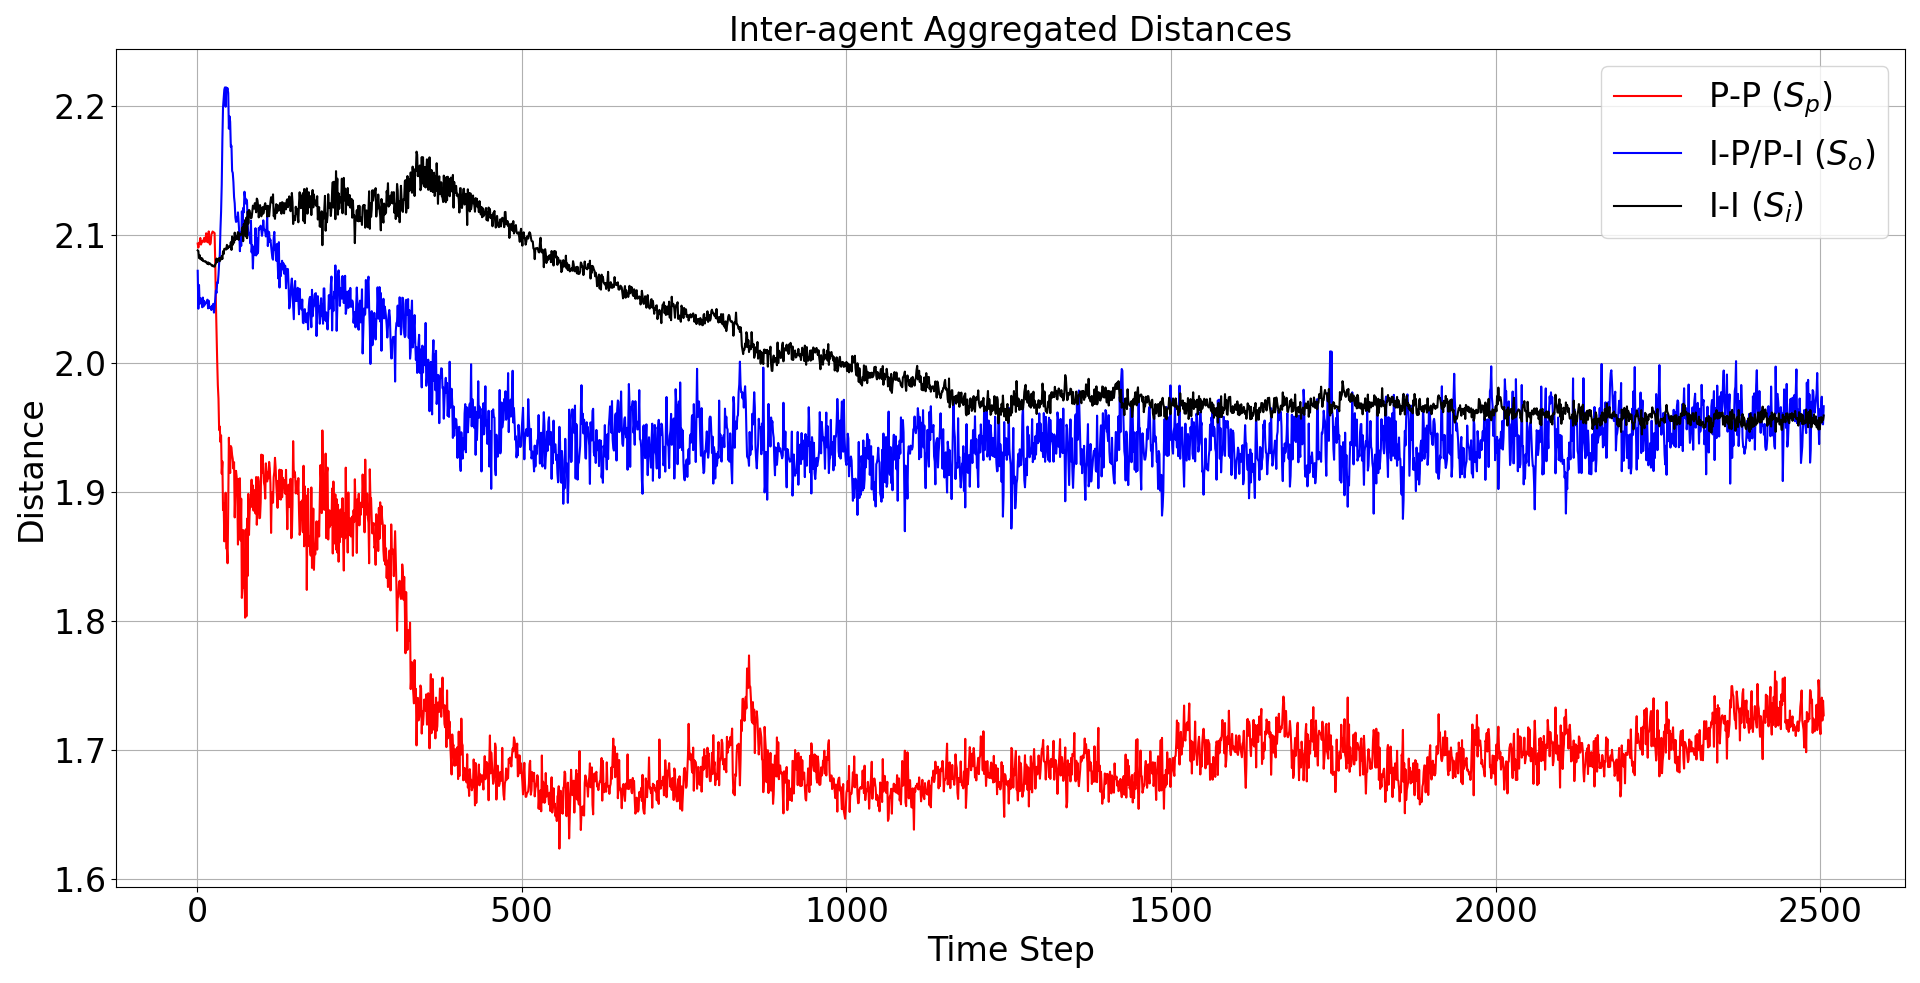
\includegraphics[width=1.0\linewidth]{figures/Future8}
	\end{center}
	\caption{Perimeter packed - Self Healing (Distance)\label{fig:future8}}
\end{figure}
%\FloatBarrier

\bibliographystyle{abbrv}
\bibliography{perimeter}

\end{document}
